% !TEX program = xelatex

\documentclass[conference]{IEEEtran}
\IEEEoverridecommandlockouts
% The preceding line is only needed to identify funding in the first footnote. If that is unneeded, please comment it out.
\usepackage{cite}
\usepackage{amsmath,amssymb,amsfonts}
\usepackage{algorithmic}
\usepackage{graphicx}
\usepackage{textcomp}
\usepackage{xcolor}
\usepackage{amsfonts,amssymb}
\usepackage{amsmath}
\usepackage{amsthm}
\usepackage[left=1.0cm,right=1.0cm,top=1.3cm,bottom=1.3cm]{geometry}
\usepackage{enumerate}
\usepackage{fancyhdr}
\usepackage{ctex}
\usepackage{xpatch}
\usepackage{graphicx} %插入图片的宏包
\usepackage{float} %设置图片浮动位置的宏包
\usepackage{subfigure} %插入多图时用子图显示的宏包
\usepackage{listings}
\usepackage{color}
\usepackage{amssymb,mathrsfs,amsmath}
\usepackage{bbding}
\usepackage{mathrsfs}

\newtheoremstyle{break}
    {\topsep}{\topsep}%
    {\itshape}{}%
    {\bfseries}{}%
    {\newline}{}%
\theoremstyle{break}

\definecolor{dkgreen}{rgb}{0,0.6,0}
\definecolor{gray}{rgb}{0.5,0.5,0.5}
\definecolor{mauve}{rgb}{0.58,0,0.82}

\lstset{frame=tb,
  language=Python,
  aboveskip=3mm,
  belowskip=3mm,
  showstringspaces=false,
  columns=flexible,
  basicstyle={\small\ttfamily},
  numbers=none,
  numberstyle=\tiny\color{gray},
  keywordstyle=\color{blue},
  commentstyle=\color{dkgreen},
  stringstyle=\color{mauve},
  breaklines=true,
  breakatwhitespace=true,
  tabsize=3
}

\def\BibTeX{{\rm B\kern-.05em{\sc i\kern-.025em b}\kern-.08em
    T\kern-.1667em\lower.7ex\hbox{E}\kern-.125emX}}
\begin{document}

\title{简易无线输电模型研究\\
{\footnotesize }
\thanks{Identify applicable funding agency here. If none, delete this.}
}

\author{\IEEEauthorblockN{Liu}
\IEEEauthorblockA{
\textit{SIST}\\
2019XXXXXX\\
XXX@shanghaitech.edu.cn}
\and
\IEEEauthorblockN{Wang}
\IEEEauthorblockA{
\textit{SIST}\\
2019XXXXXX\\
XXX@shanghaitech.edu.cn}
\and
\IEEEauthorblockN{Qin}
\IEEEauthorblockA{
\textit{SIST}\\
2019XXXXXX\\
XXX@shanghaitech.edu.cn}
}

\maketitle

\begin{abstract}
        本研究基于简易自制自激振荡模块,手制漆包线电磁感应线圈,LED灯,辅以单片机与配套模块与传感器,通过控制变量法进行对于影响无线输电特性的五个因素的探究,并用示波器进行定量测量,得出了一系列定性结论。同时小组成员就霍尔传感器电机测速实验进行探究,完成了一个基于Arduino单片机的霍尔测速器。
\end{abstract}

\begin{IEEEkeywords}
        自激振荡电路   无线输电 
\end{IEEEkeywords}

\section{实验目的}
\begin{itemize}
        \item 探究无线输电特性的五个因素: 电压,频率,线圈直径,线圈匝数,发射线圈与接收线圈之间的角度
        \item 采用计算机程序拟合长冈系数,从而计算出线圈电感,进行无线输电频率因素探究
        \item 采用计算机程序拟合长冈系数,从而计算出线圈电感,进行无线输电频率因素探究
\end{itemize}

\section{实验原理}
本实验主要应用以下三个物理规律:
\begin{enumerate}
        \item 电流的磁效应:任何通有电流的导线,都可以在其周围产生磁场的现象
        \item 电磁感应:放在变化	磁通量中的导体,会产生电动势。此电动势称为感应电动势,若将此导体闭合成一回路,则该电动势会驱使电子流动,形成	感应电流。
        \item 自激振荡电路:接通电源瞬间,由于电路的扰动,放大器输入端得到一个信号,到输出端就z被放大了许多倍,输出端的这个大信号又被送到输入端,到输出端就变得更大,如此周而复始,信号越来越大,大到放大器的非线性出现,信号才会稳定在一定的幅度输出。如此就得到稳定的自激输出。这就是自激震荡产生的过程
\end{enumerate}
\section{准备工作}

\subsection{基础实验器材}

\begin{itemize}
        \item 游标卡尺与直尺
        \item 直径为0.49mm的漆包线500g
        \item 铝制支架与铁质滑轨(为方便起见,下文统称铁芯)
        \item 自激振荡电路
        \item 发光二极管
        \item 导线与电路连接元件
        \item KEYSIGHT DSOS104A 示波器
\end{itemize}
\begin{figure}[htbp]
        \centerline{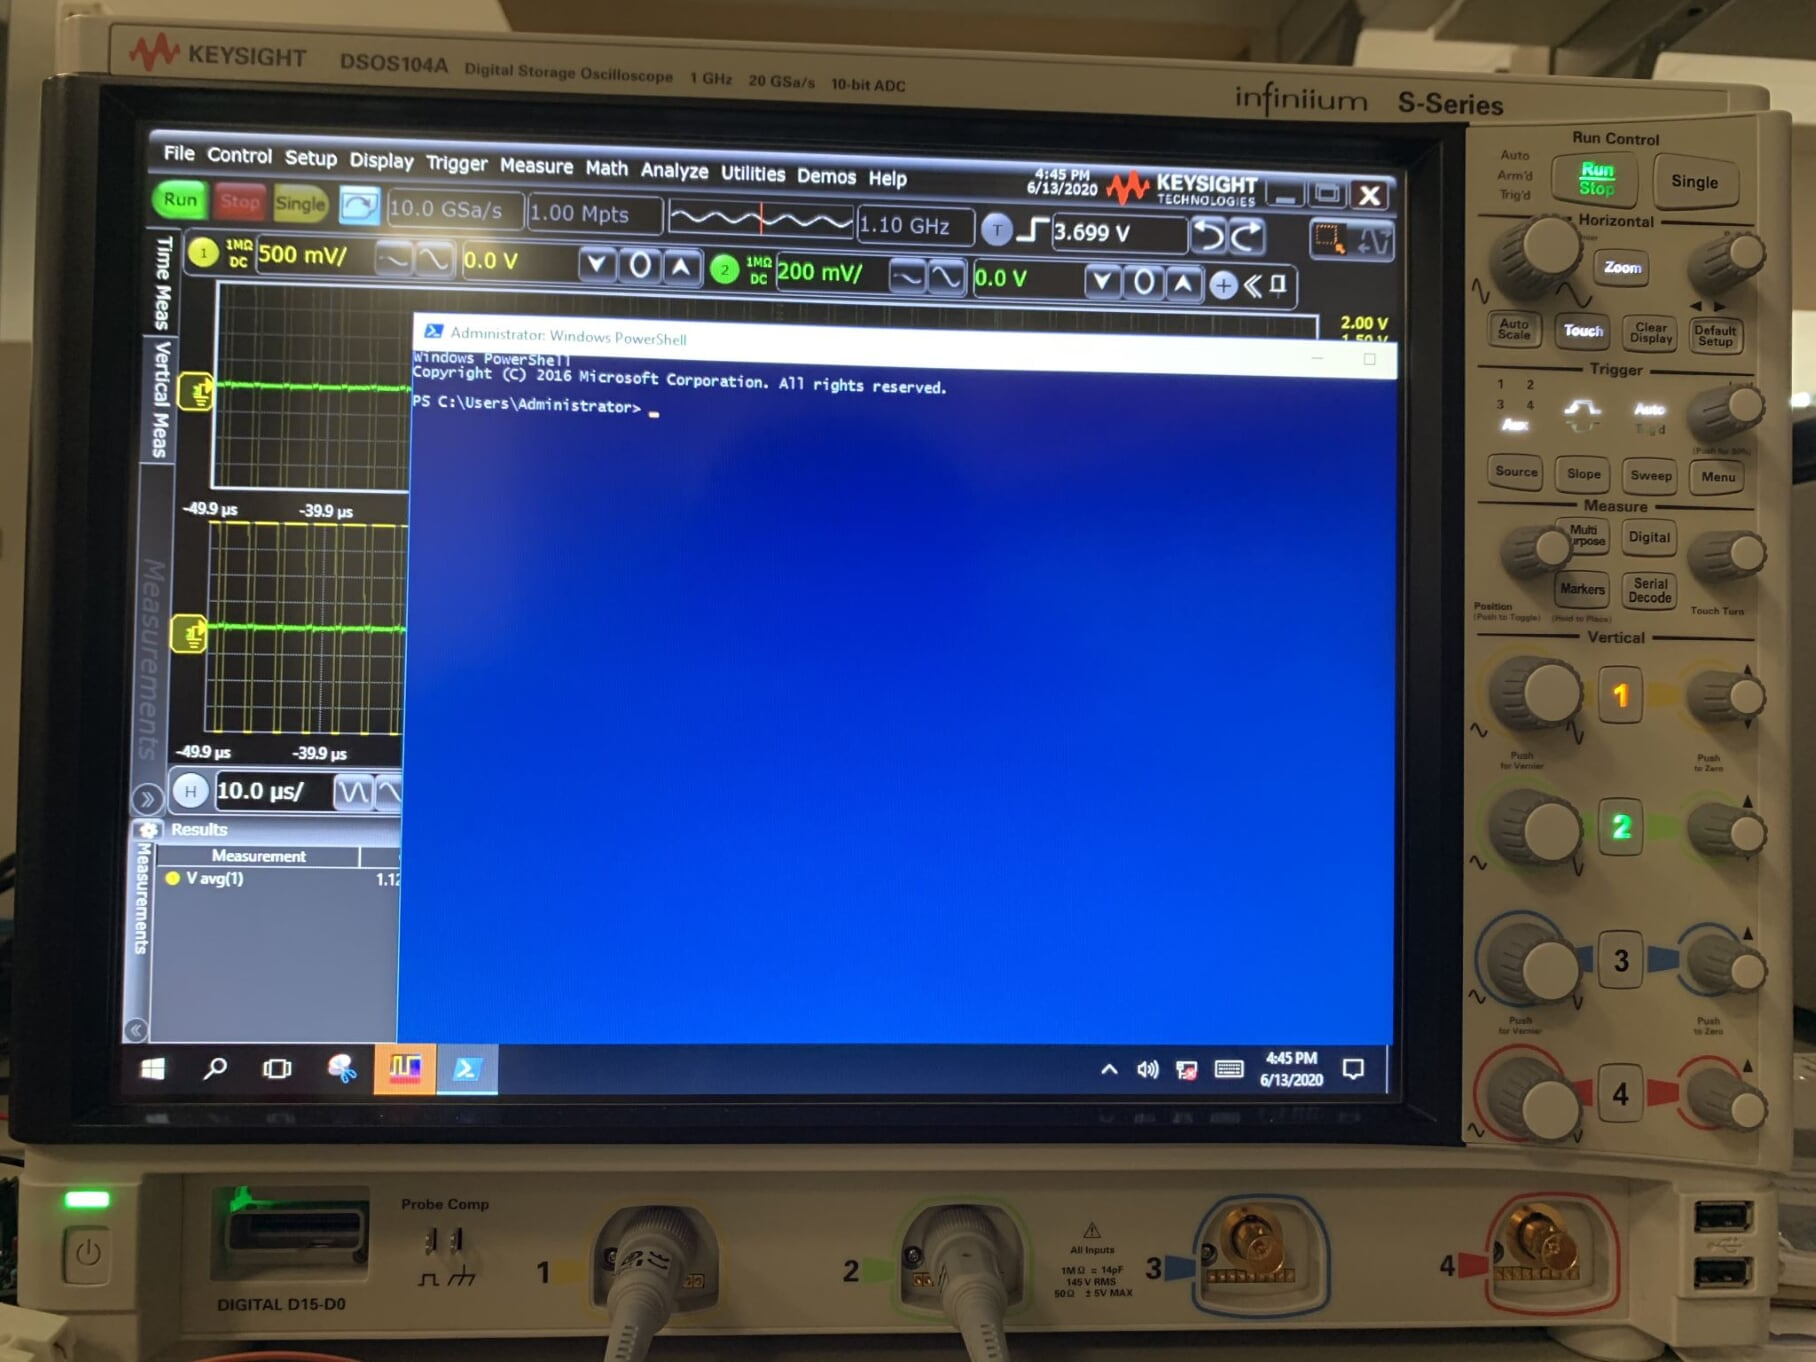
\includegraphics[scale=0.1]{示波器.JPG}}
        \caption{EYSIGHT DSOS104A示波器}
        \label{fig}
        \end{figure}
\subsection{单片机与模块}
\subsubsection{Arduino R3 兼容板}
该兼容版提供了pwn输出,模拟输入和输出,数字输入和输出,并通过串口连接计算机,可以提供串口通信和根据串口通信值进行绘图操作。
在本实验中,该兼容版负责连接距离传感器,霍尔传感器等,并进行串口输出。
\subsubsection{超声波距离传感器 HC-SR04}
该模块包含超声波发生器,接收器,与控制电路,可提供2-200cm的非接触式距离感测功能,测距精度可达3mm。
\begin{figure}[htbp]
        \centerline{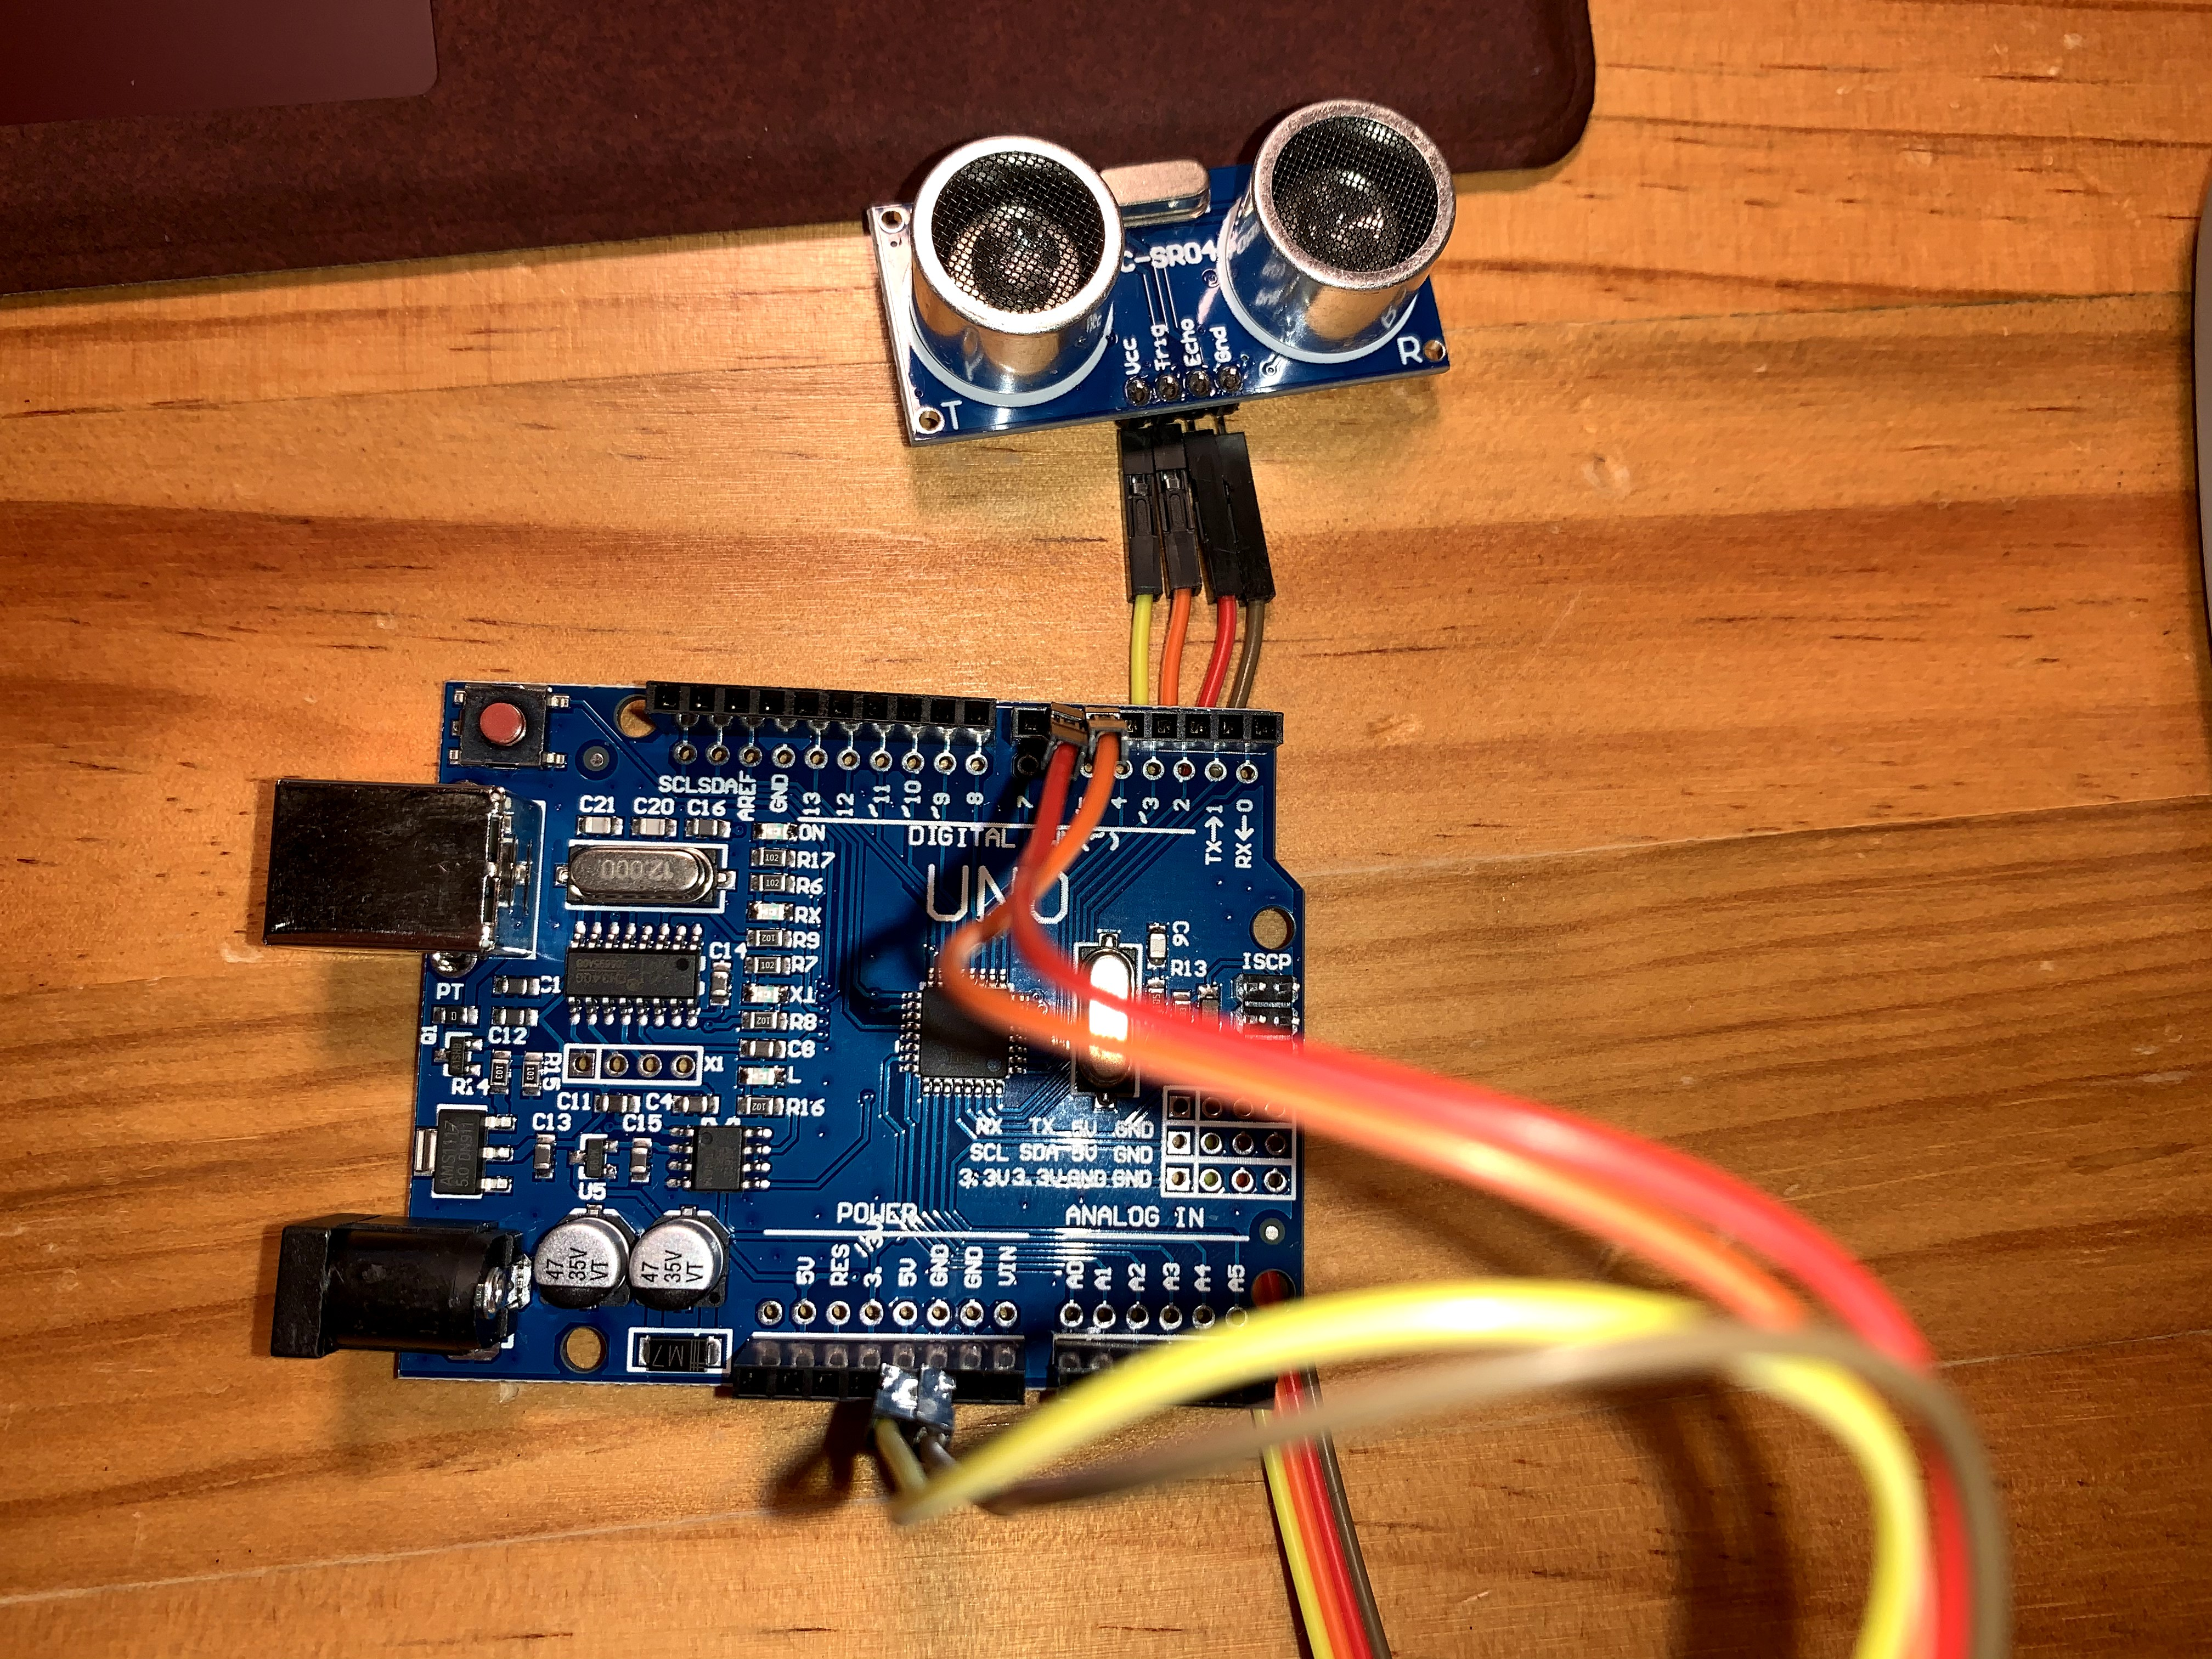
\includegraphics[scale=0.05]{超声波传感器.JPG}}
        \caption{超声波距离传感器与电路搭建}
        \label{fig}
        \end{figure}
        \begin{figure}[htbp]
                \centerline{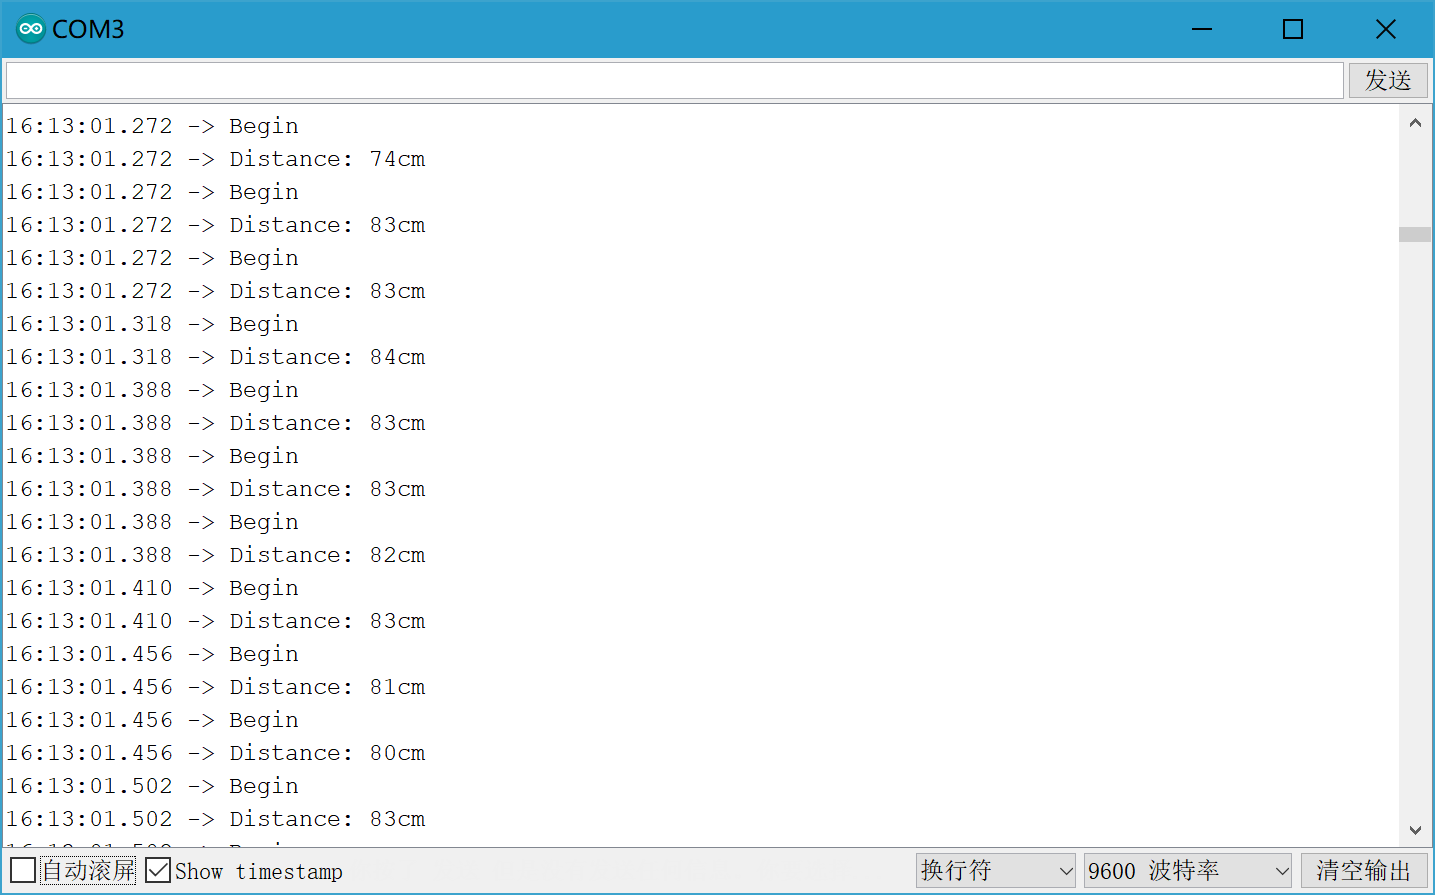
\includegraphics[scale=0.17]{距离传感器输出样例.png}}
                \caption{超声波距离传感器输出样例}
                \label{fig}
                \end{figure}
\\
\textbf{工作原理}
\begin{itemize}
        \item 采用IO口TRIG触发测距,产生至少10us的高电平信号
        \item 模块自动发送8个40khz的方波,自动检测是否有信号返回
        \item 有信号返回,通过IO口ECHO输出一个高电平,高电平持续的时间就是超声波从发射到返回的时间。
\end{itemize}
距离 = $\frac{The\ time\ period\ of\ HIGH\ output \cdot SOUND\ SPEED}{2}$\\
\textbf{代码见附录}

\subsubsection{3144 霍尔元件}
A3144E霍尔元件44E OH44E 霍尔传感器霍尔开关集成电路应用霍尔效应原理,采用半导体集成技术制造的磁敏电路,它是由电压调整器、霍尔电压发生器、差分放大器、史密特触发器,温度补偿电路和集电极开路的输出级组成的磁敏传感电路,其输入为磁感应强度,输出是一个数字电压讯号。
\begin{figure}[htbp]
        \centerline{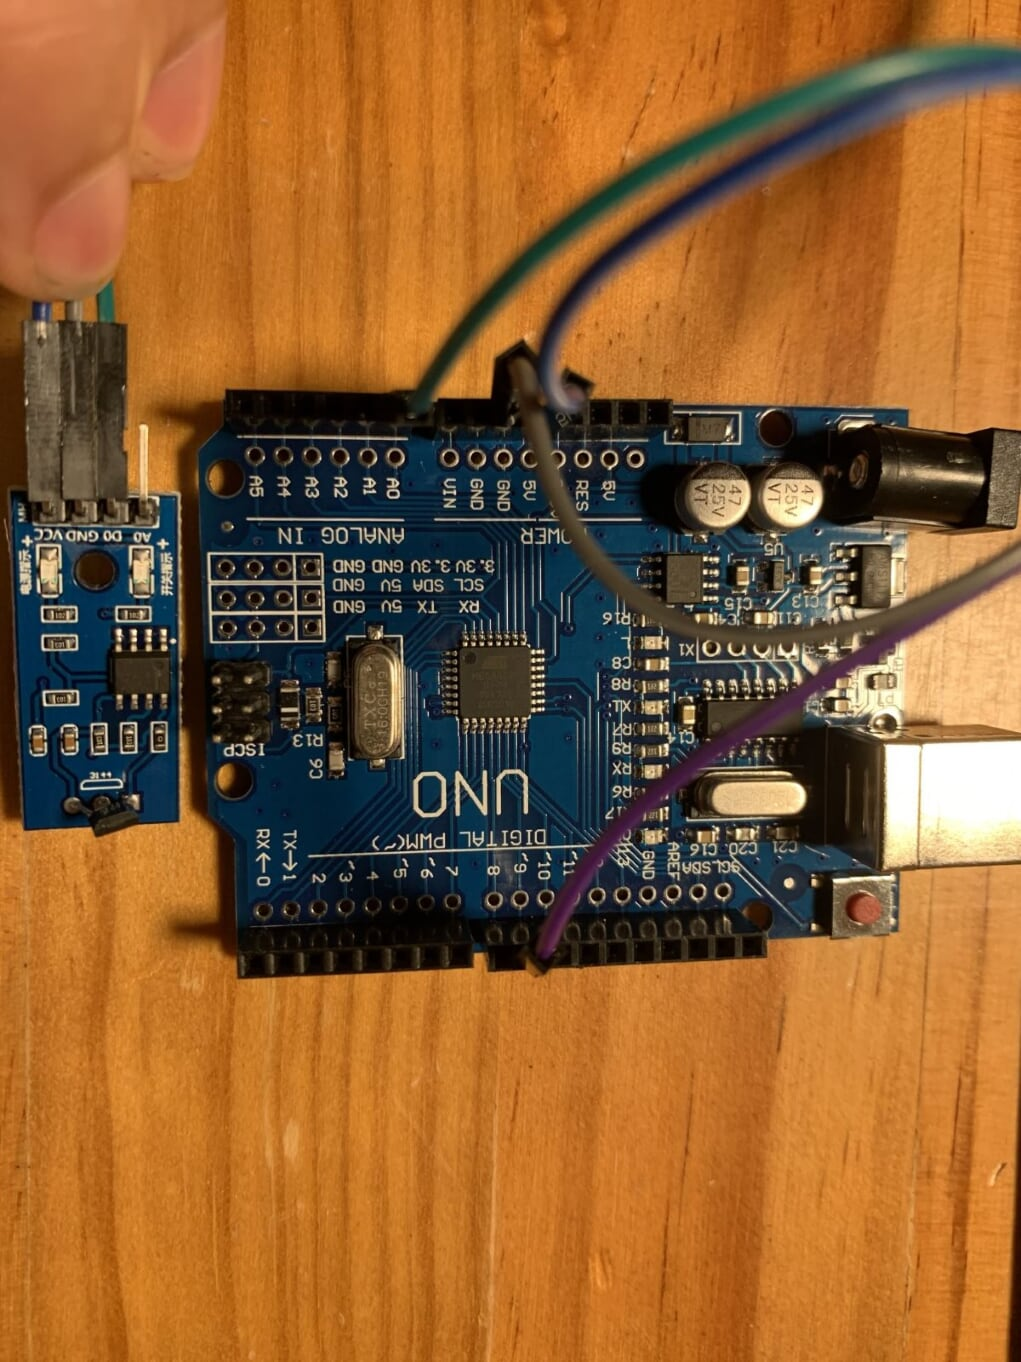
\includegraphics[scale=0.1]{非线性霍尔.JPG}}
        \caption{非线性霍尔传感器3144}
        \label{fig}
        \end{figure}

\subsubsection{49E 线性霍尔元件}
S49E系列线性霍尔电路由电压调整器,霍尔电压发生器,线性放大器和射极跟随器组成,其输入是磁感应强度,输出是和输入量成正比的电压。
\begin{figure}[htbp]
        \centerline{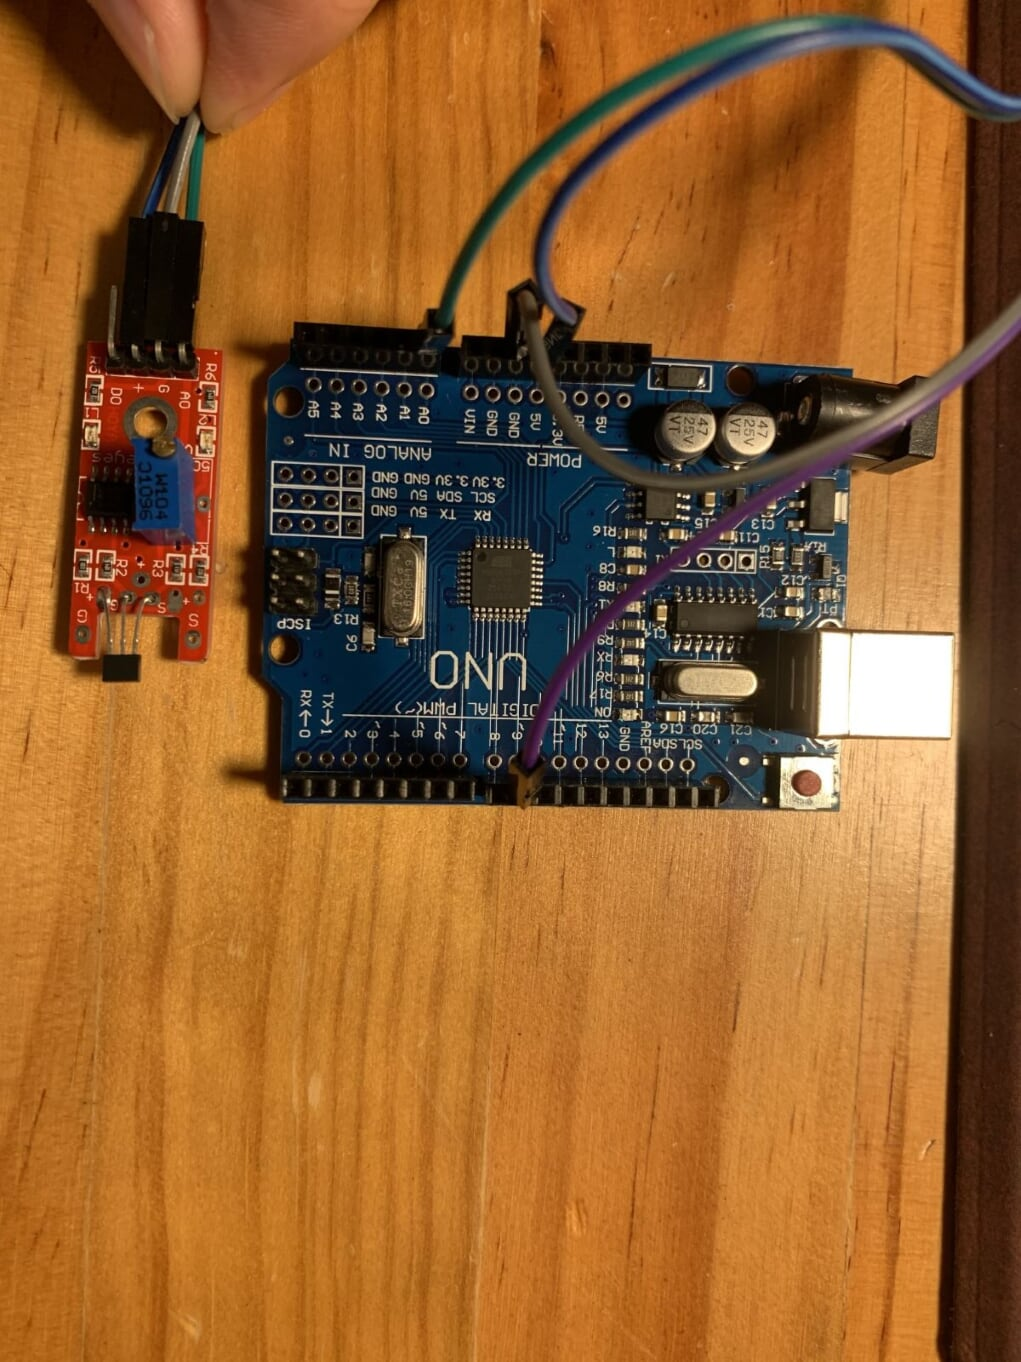
\includegraphics[scale=0.1]{线性霍尔.JPG}}
        \caption{线性霍尔传感器49E}
        \label{fig}
        \end{figure}
        \begin{figure}[htbp]
                \centerline{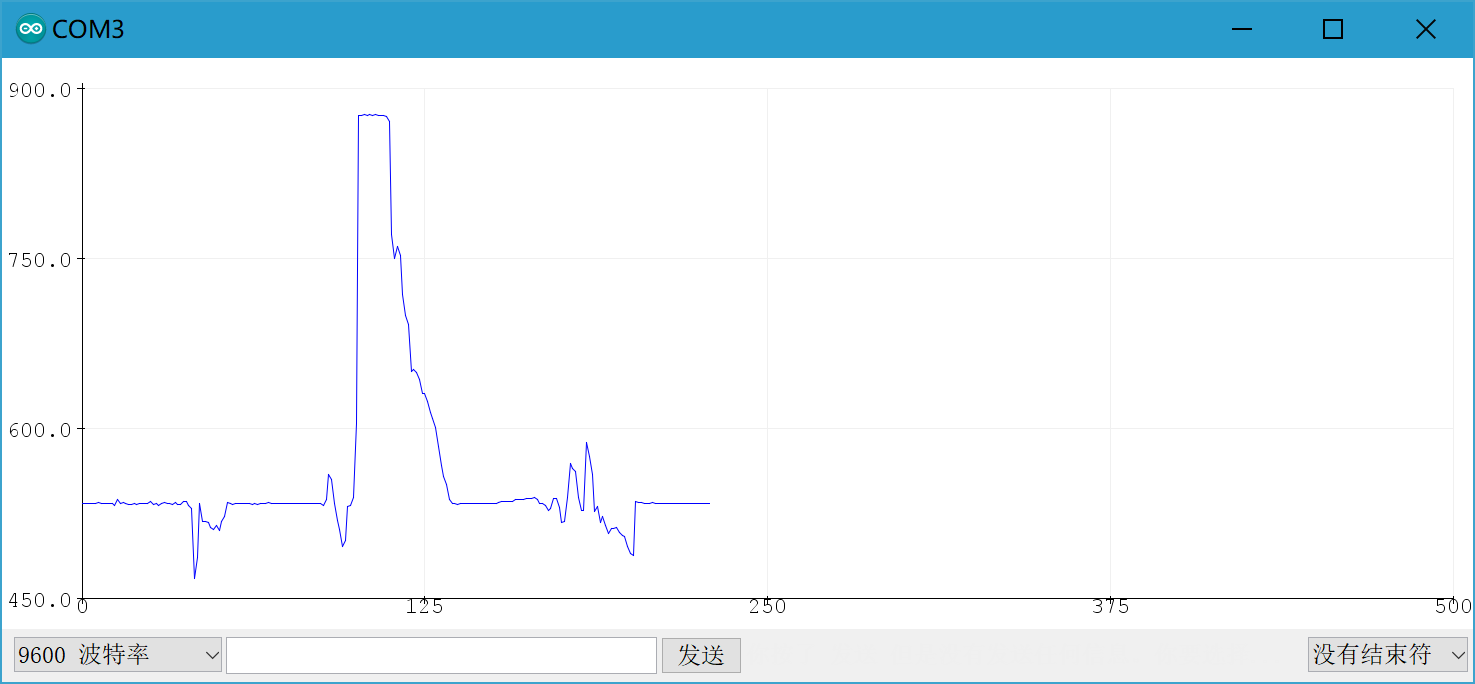
\includegraphics[scale=0.1]{霍尔输出.png}}
                \caption{线性霍尔传感器输出样例-当磁铁靠近后远离}
                \label{fig}
                \end{figure}
\\
\textbf{代码见附录}
\subsubsection{霍尔元件的选择}
3144为非线性霍尔元件,当磁通量超过阈值时输出一个高电平,而49E为线性霍尔元件,输出电压与磁通量成正比,输出信号为模拟信号(0 - 1024)。
因此在做霍尔电机测速器时可以选择线性与非线性的霍尔传感器。而如果要定量测量磁通量,则需要选择线性的霍尔传感器49E。

\subsection{发射线圈}
考虑实验过程的方便,我们组决定制作一个可以直立,并且方便旋转,中心对称且旋转对称。所以我们组用Adobe Inventor软件进行3D建模,导出stl文件后利用3D打印机进行发射线圈的制作。\\
为了控制发射线圈的直径与匝数,我们分别制作了3个发射线圈,分别是:

\begin{table}[htbp]
        \caption{发射线圈参数表}
        \begin{center}
        \begin{tabular}{|c|c|c|c|}
        \hline
        \textbf{线圈编号}&\textbf{直径} & \textbf{匝数}& \textbf{颜色} \\
        \hline
        发射线圈A&3cm&15&黄\\
        \hline
        发射线圈B&8cm&10&绿\\
        \hline
        发射线圈C&8cm&15&黄\\
        \hline
        \end{tabular}
        \label{tab1}
        \end{center}
        \end{table}

\begin{figure}[htbp]
        \centerline{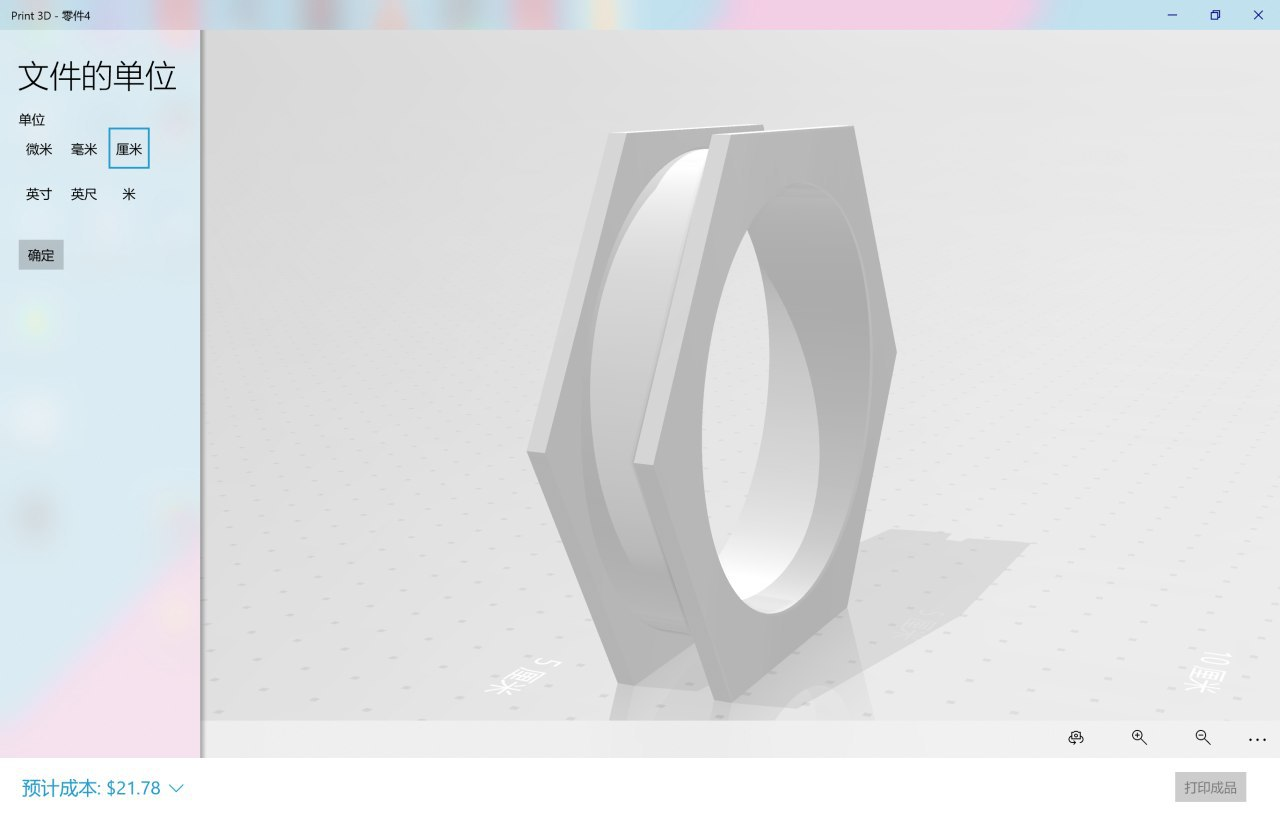
\includegraphics[scale=0.1]{发射线圈1.png}}
        \caption{.stl格式的发射线圈C建模图}
        \label{fig}
        \end{figure}
\begin{figure}[htbp]
        \centerline{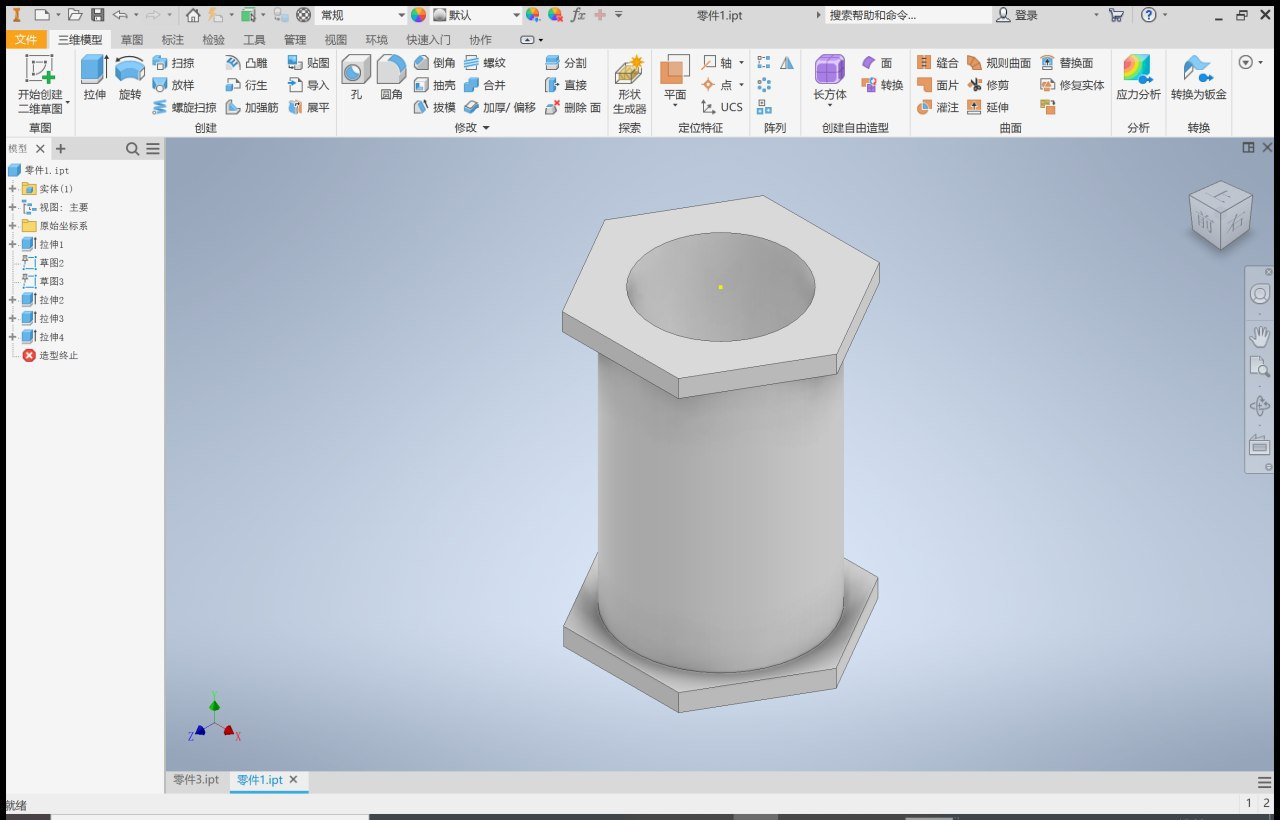
\includegraphics[scale=0.1]{发射线圈2.png}}
        \caption{发射线圈A的建模过程}
        \label{fig}
        \end{figure}
\begin{figure}[htbp]
        \centerline{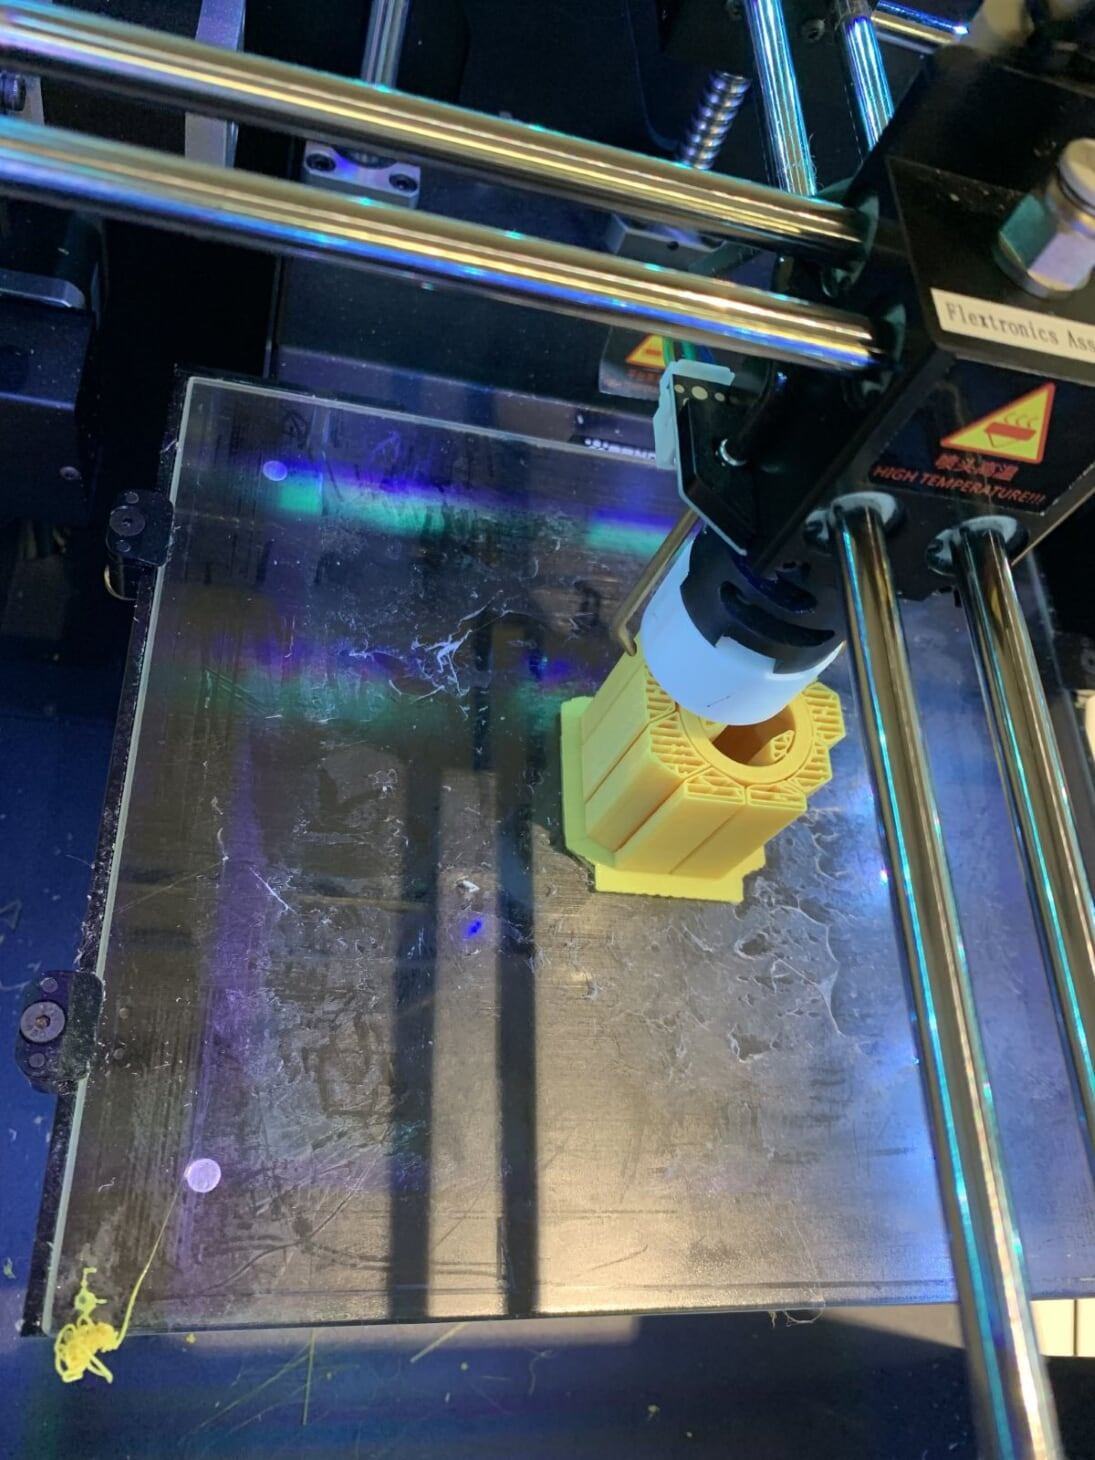
\includegraphics[scale=0.1]{发射线圈打印.png}}
        \caption{发射线圈A的3D打印过程}
        \label{fig}
        \end{figure}
\begin{figure}[htbp]
        \centerline{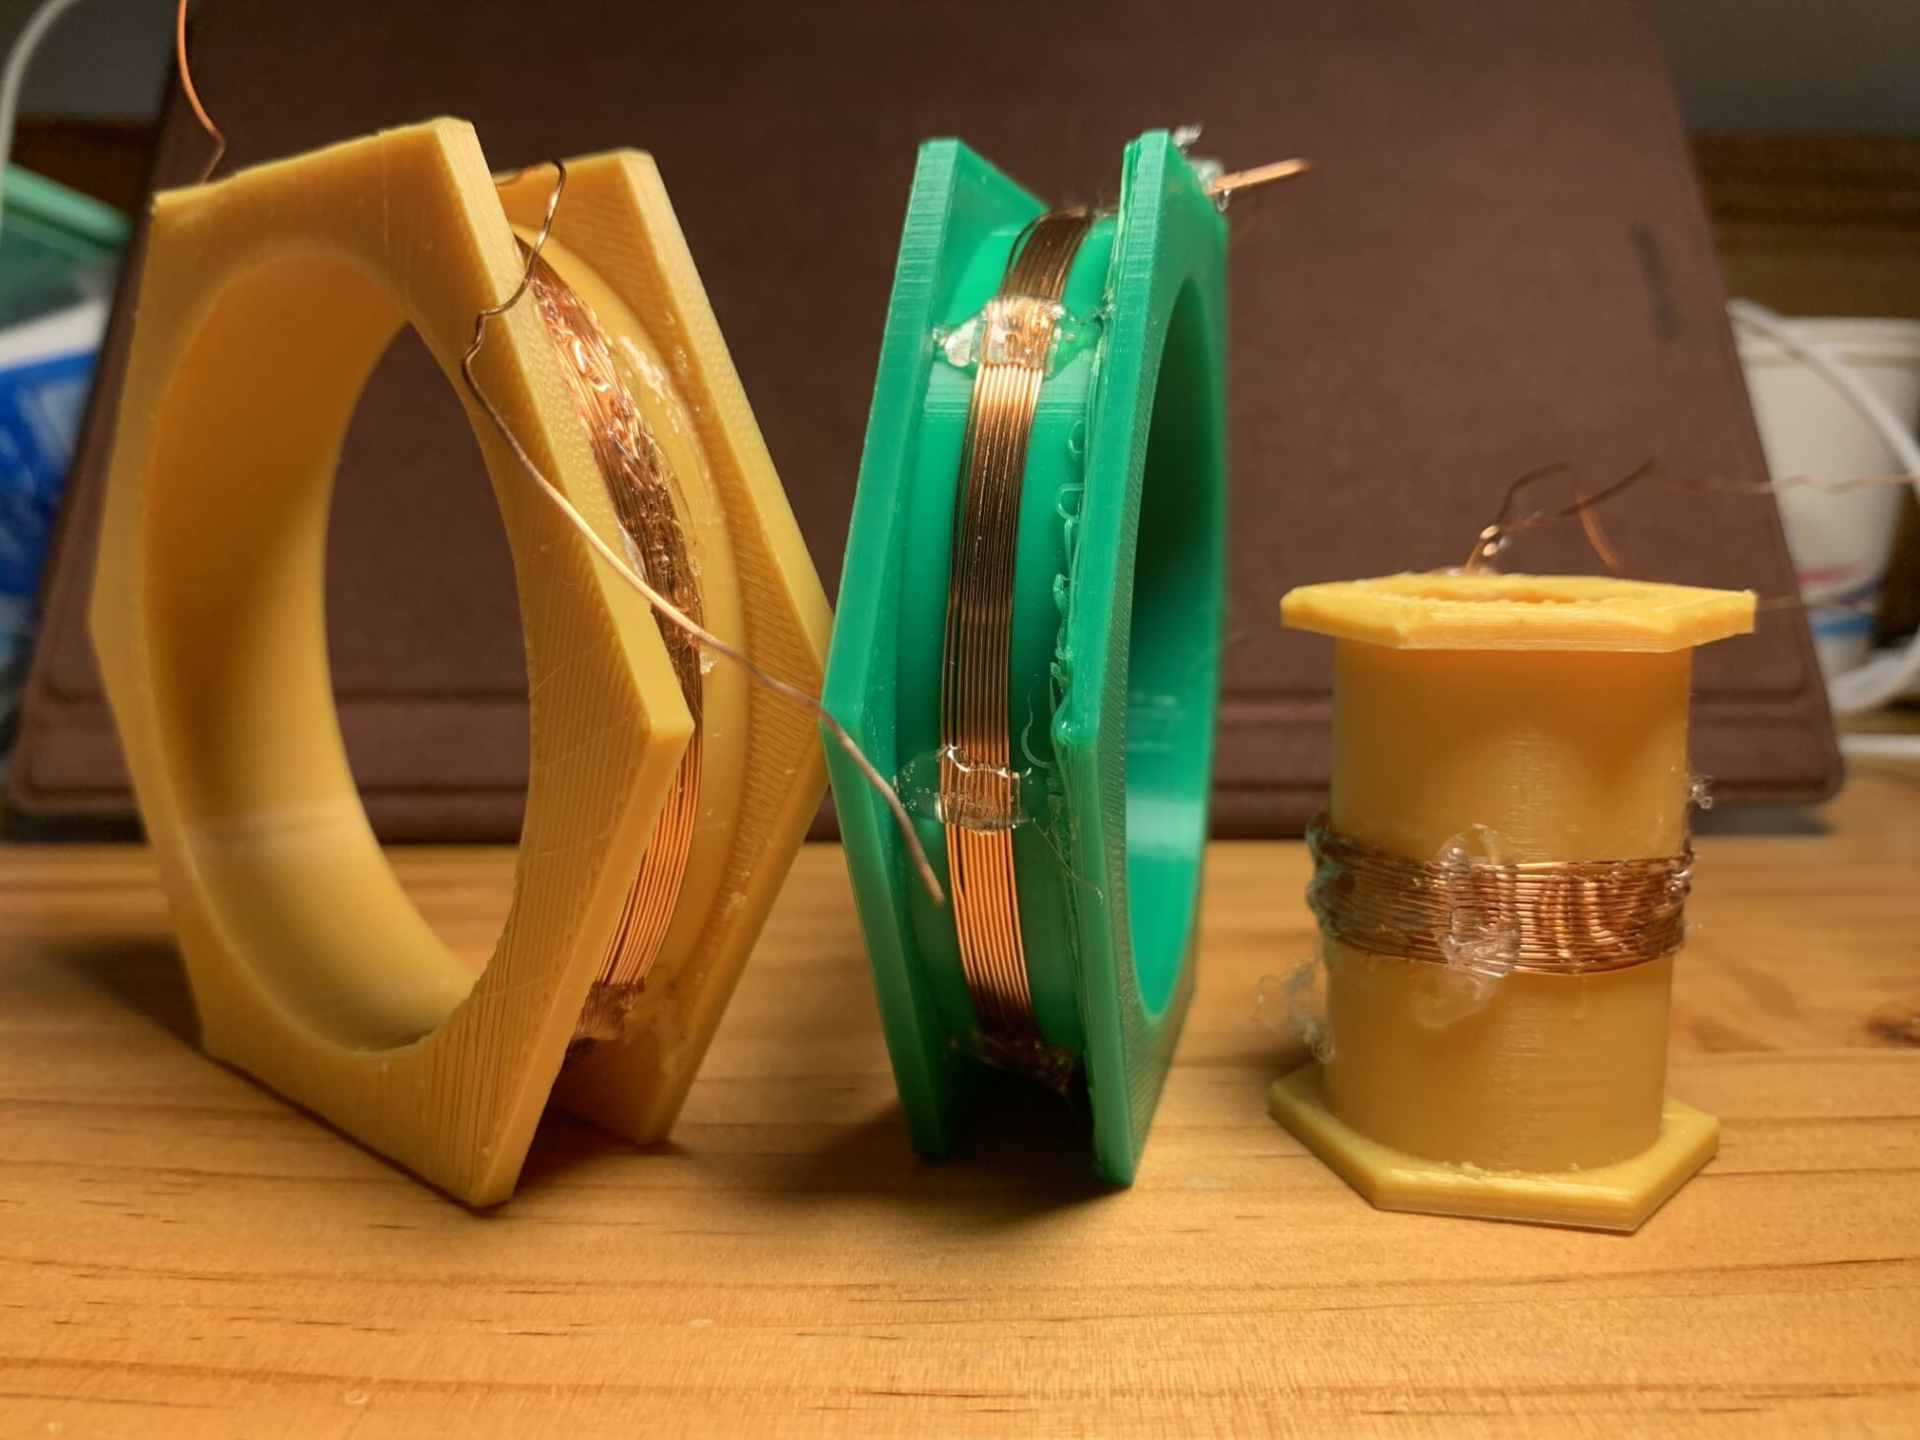
\includegraphics[scale=0.1]{发射线圈全家福.png}}
        \caption{全体发射线圈}
        \label{fig}
        \end{figure}
\leavevmode\\
\subsection{接收线圈}
接受线圈由漆包线绕制而成,载体为爱夸与贝纳颂饮料瓶以控制变量。

\begin{table}[htbp]
        \caption{发射线圈参数表}
        \begin{center}
        \begin{tabular}{|c|c|c|c|}
        \hline
        \textbf{线圈编号}&\textbf{直径} & \textbf{匝数}& \textbf{载体} \\
        \hline
        接收线圈A	&5.1cm	&15&	贝纳颂\\
        \hline
        接收线圈B	&6.3cm	&15	&爱夸\\
        \hline
        接收线圈C	&6.3cm	&30	&爱夸\\
        \hline 
        接收线圈D	&6.3cm&	60	&爱夸\\
        \hline
        \end{tabular}
        \label{tab1}
        \end{center}
        \end{table}

        \begin{figure}[htbp]
                \centerline{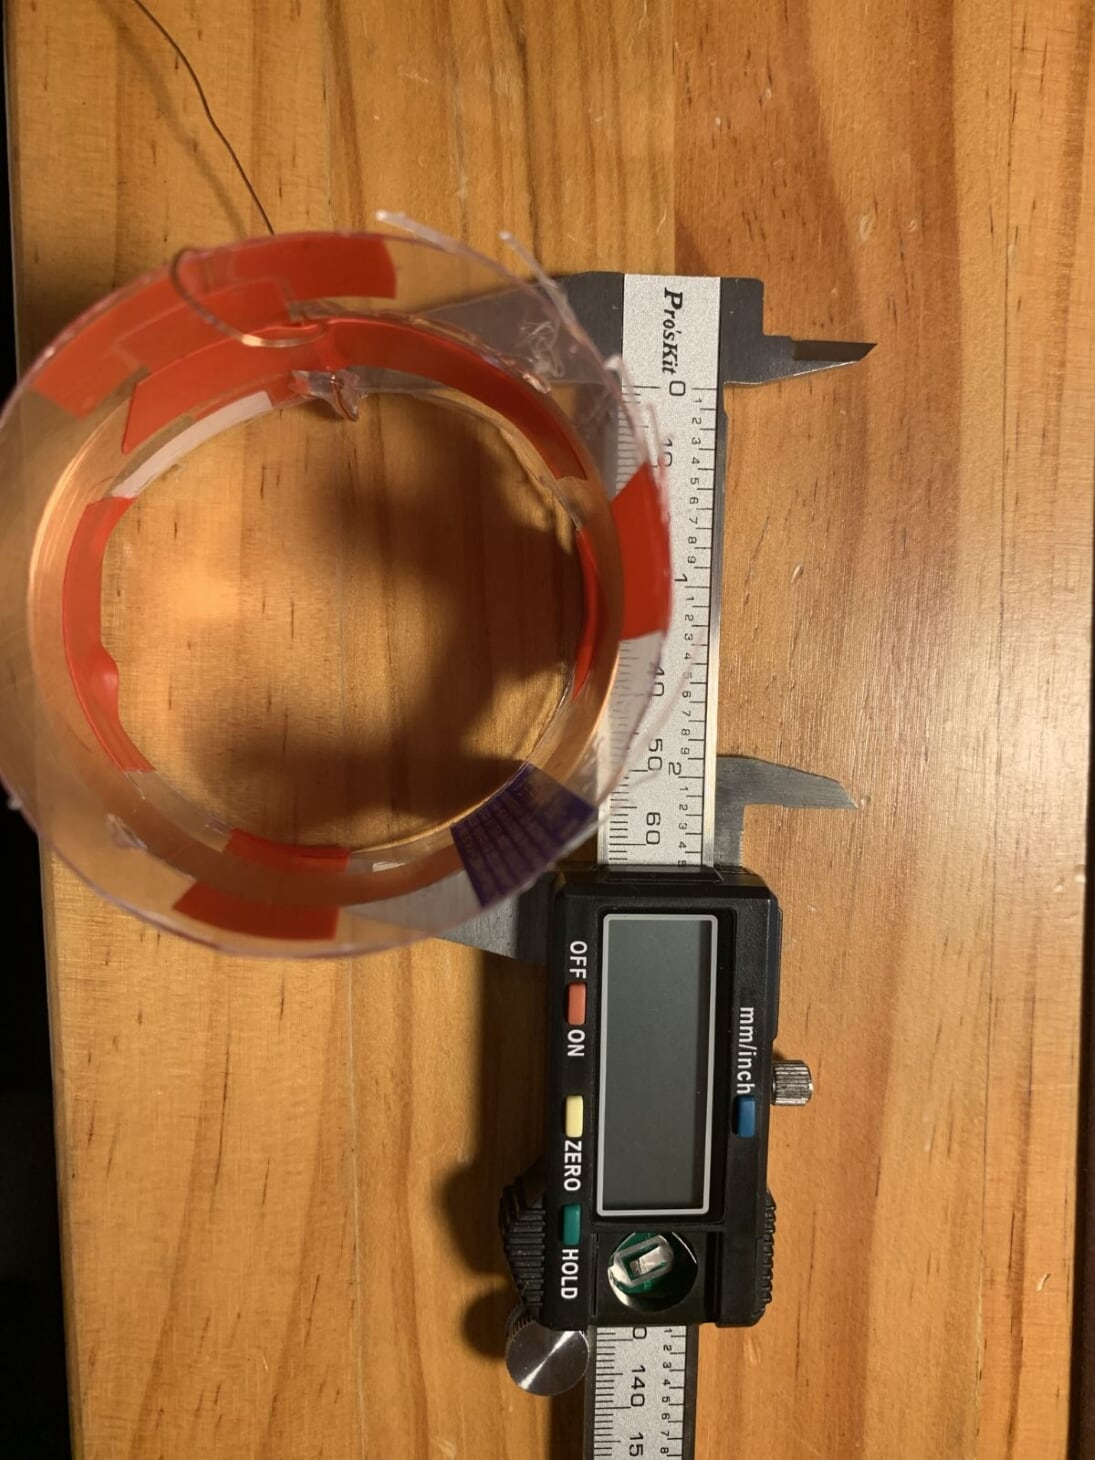
\includegraphics[scale=0.1]{接收线圈测量过程.png}}
                \caption{接收线圈测量过程}
                \label{fig}
                \end{figure}
        
        \begin{figure}[htbp]
                \centerline{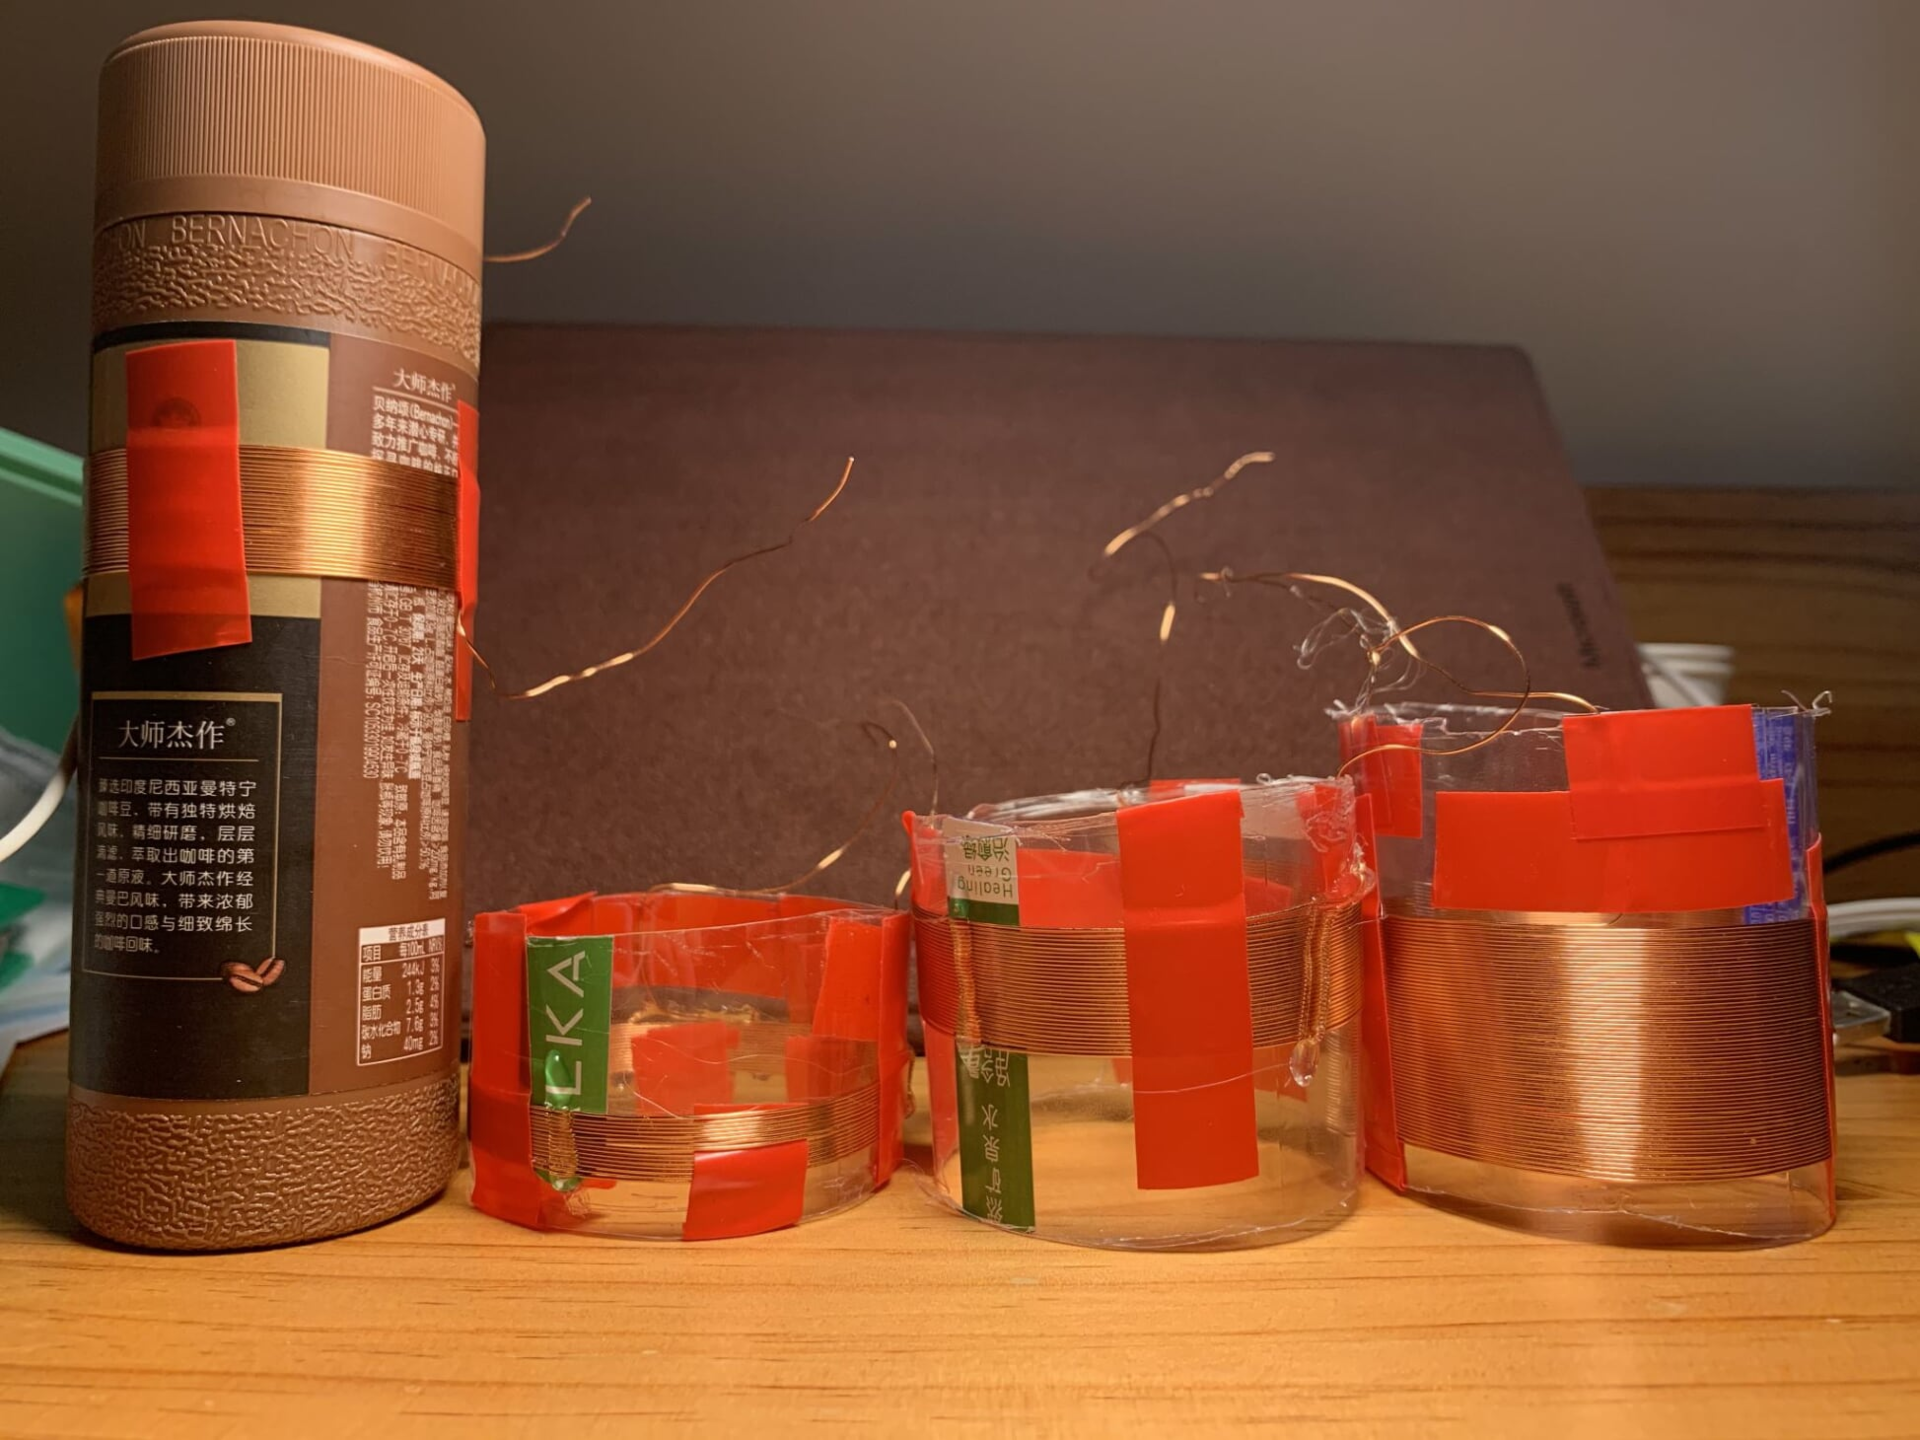
\includegraphics[scale=0.1]{接收线圈全家福.png}}
                \caption{全体接收线圈}
                \label{fig}
                \end{figure}
   
\subsection{其它}
\begin{itemize}
        \item 面包板    
        \item 杜邦线
\end{itemize}

\section{实验过程}
\subsection{控制变量:电压}
\subsubsection{实验设计}
本实验诣在探索发射线圈产生的电压正负对无线输电的影响,依据控制变量的原则设计对照实验,只改变线圈朝向。\\
\textbf{实验器材:}
\begin{itemize}
        \item 发射端:直径8cm、10匝线圈
        \item 直径6.3cm、60匝线圈、爱夸6.3cm
        \item 示波器
\end{itemize}
\subsubsection{实验过程}
控制发射端与接收端的距离为3cm,示波器与接收端线圈相连,交换发射端线圈的朝向,观察示波器的示数
\subsubsection{实验分析}
通过实验我们发现,发射端线圈正向的电压高于发射端线圈反向的电压
\subsubsection{实验结论}
\begin{figure}[htbp]
        \centerline{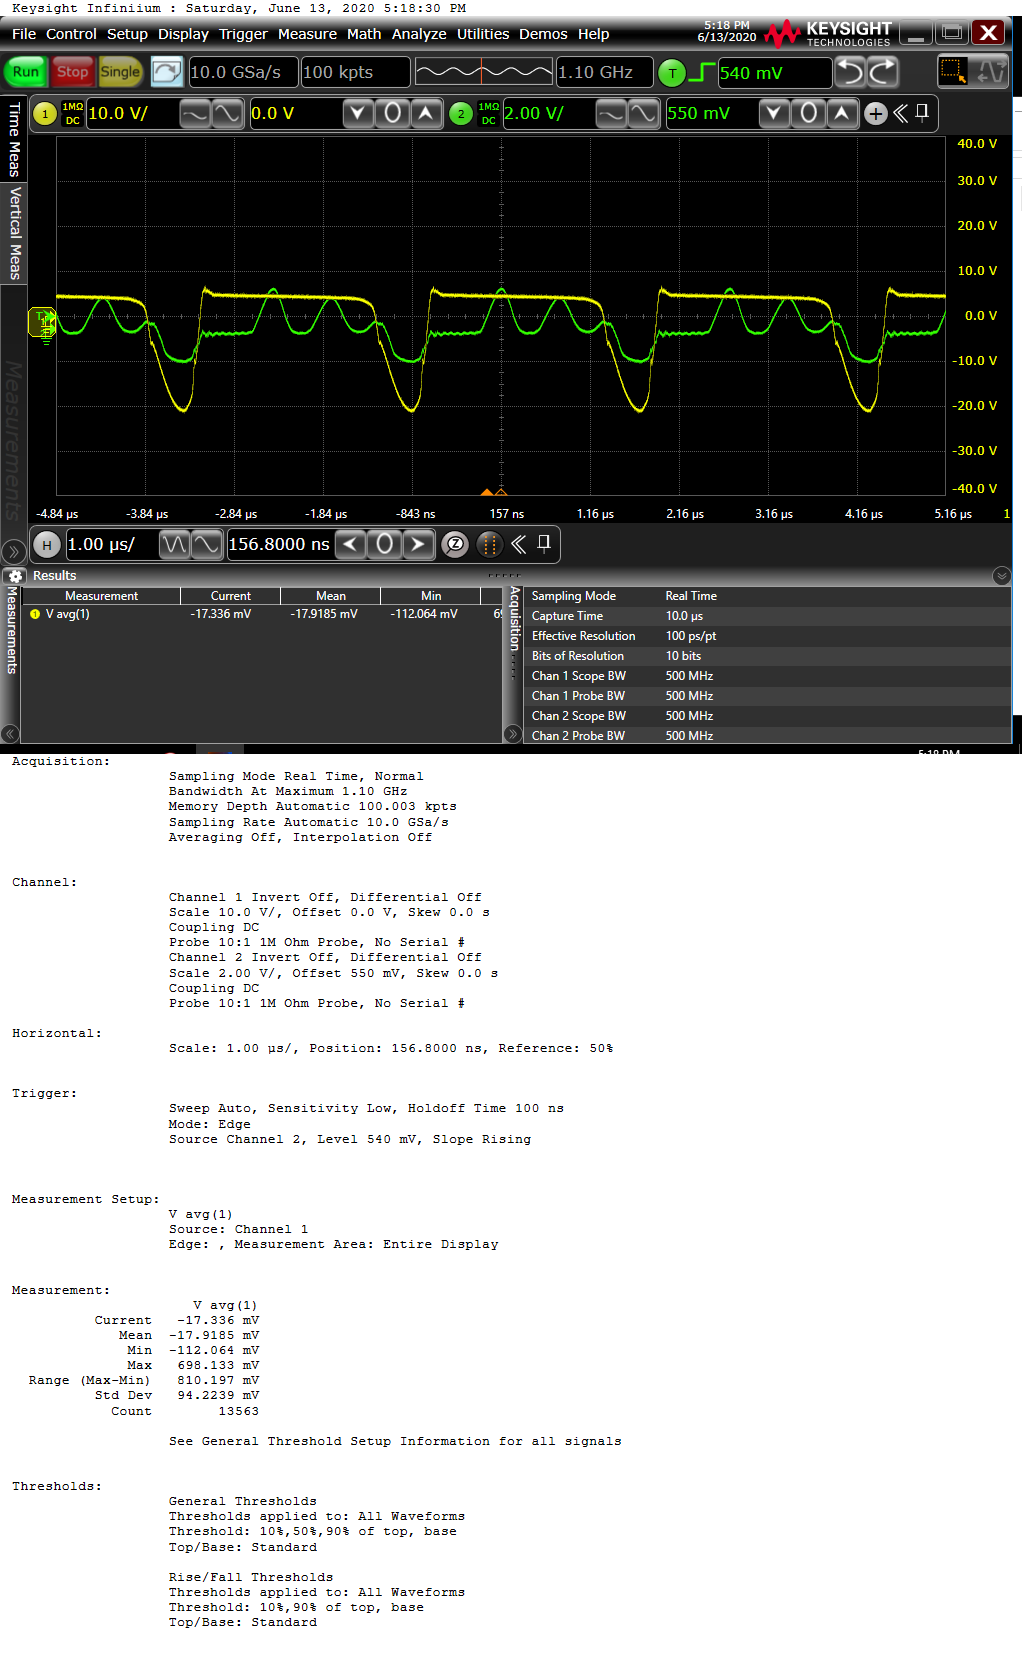
\includegraphics[scale=0.1]{电压结论1.png}}
        \caption{正向}
        \label{fig}
        \end{figure}

\begin{figure}[htbp]
        \centerline{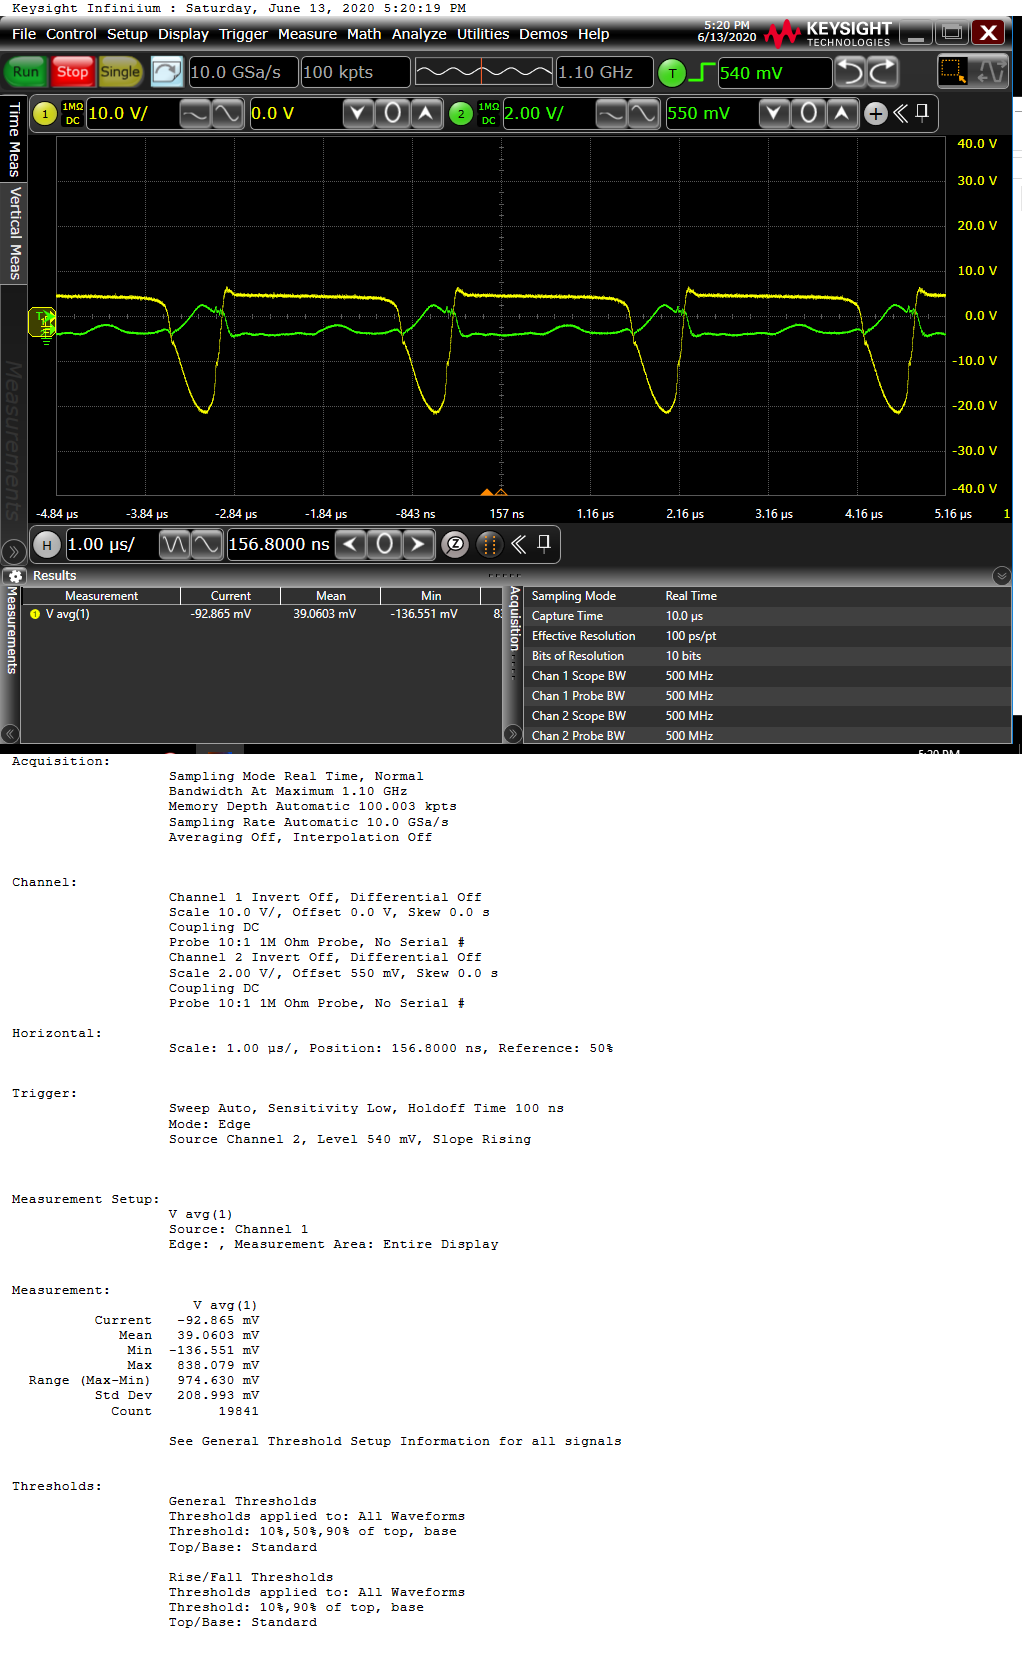
\includegraphics[scale=0.1]{电压结论2.png}}
        \caption{反向}
        \label{fig}
        \end{figure}
发射端线圈正向时可以提升无限输电的能力()

\subsection{控制变量:频率}
\subsubsection{实验设计}
本实验诣在探索发射线圈自身的频率对无线输电的影响,依据控制变量原则设计对照实验,只改变条件——插入铁芯。 \\
\textbf{实验器材:}
\begin{itemize}
        \item 发射端:直径8cm、15匝线圈
        \item 接收端:直径6.3cm、30匝线圈
        \item 示波器
        \item 铁芯
\end{itemize}
\subsection{实验过程}
控制距离3.5cm,分别观察两组实验中示波器的示数
\subsection{实验分析}
通过实验我们发现,插入铁芯组的电压高于没有插入铁芯组的电压
\subsection{实验结论}
在一定范围内提高发射端的频率可以提高无线输电的能力
\begin{figure}[htbp]
        \centerline{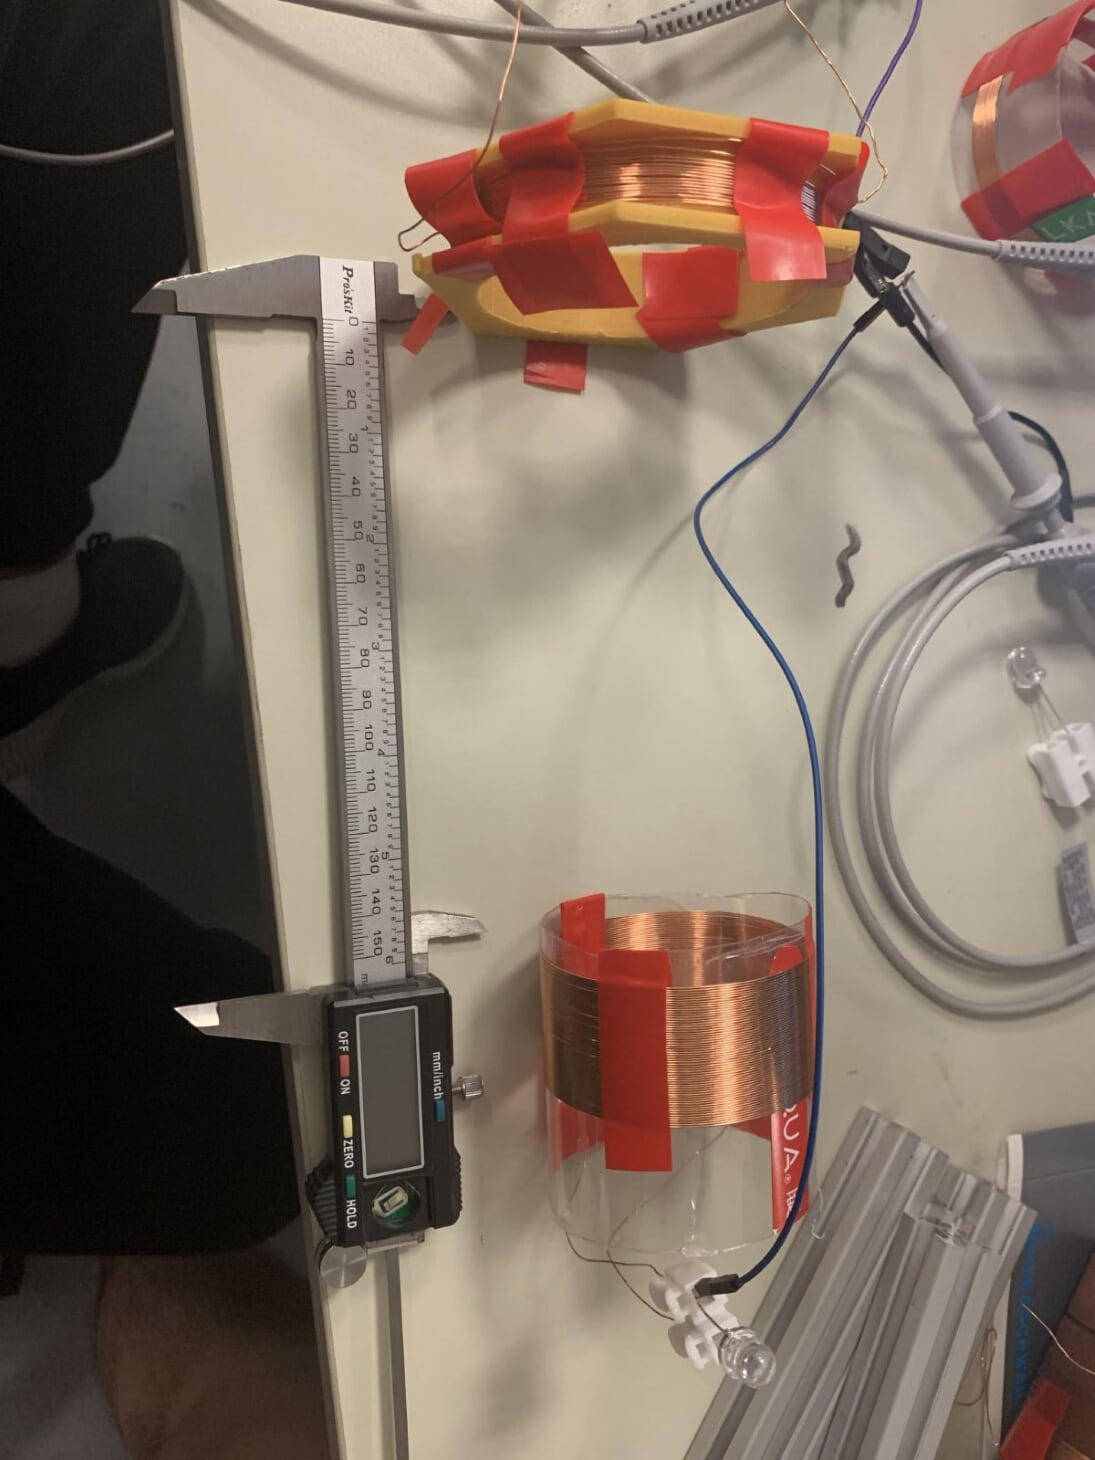
\includegraphics[scale=0.1]{频率1.png}}
        \caption{控制距离不变,不插铁芯}
        \label{fig}
        \end{figure}

\begin{figure}[htbp]
        \centerline{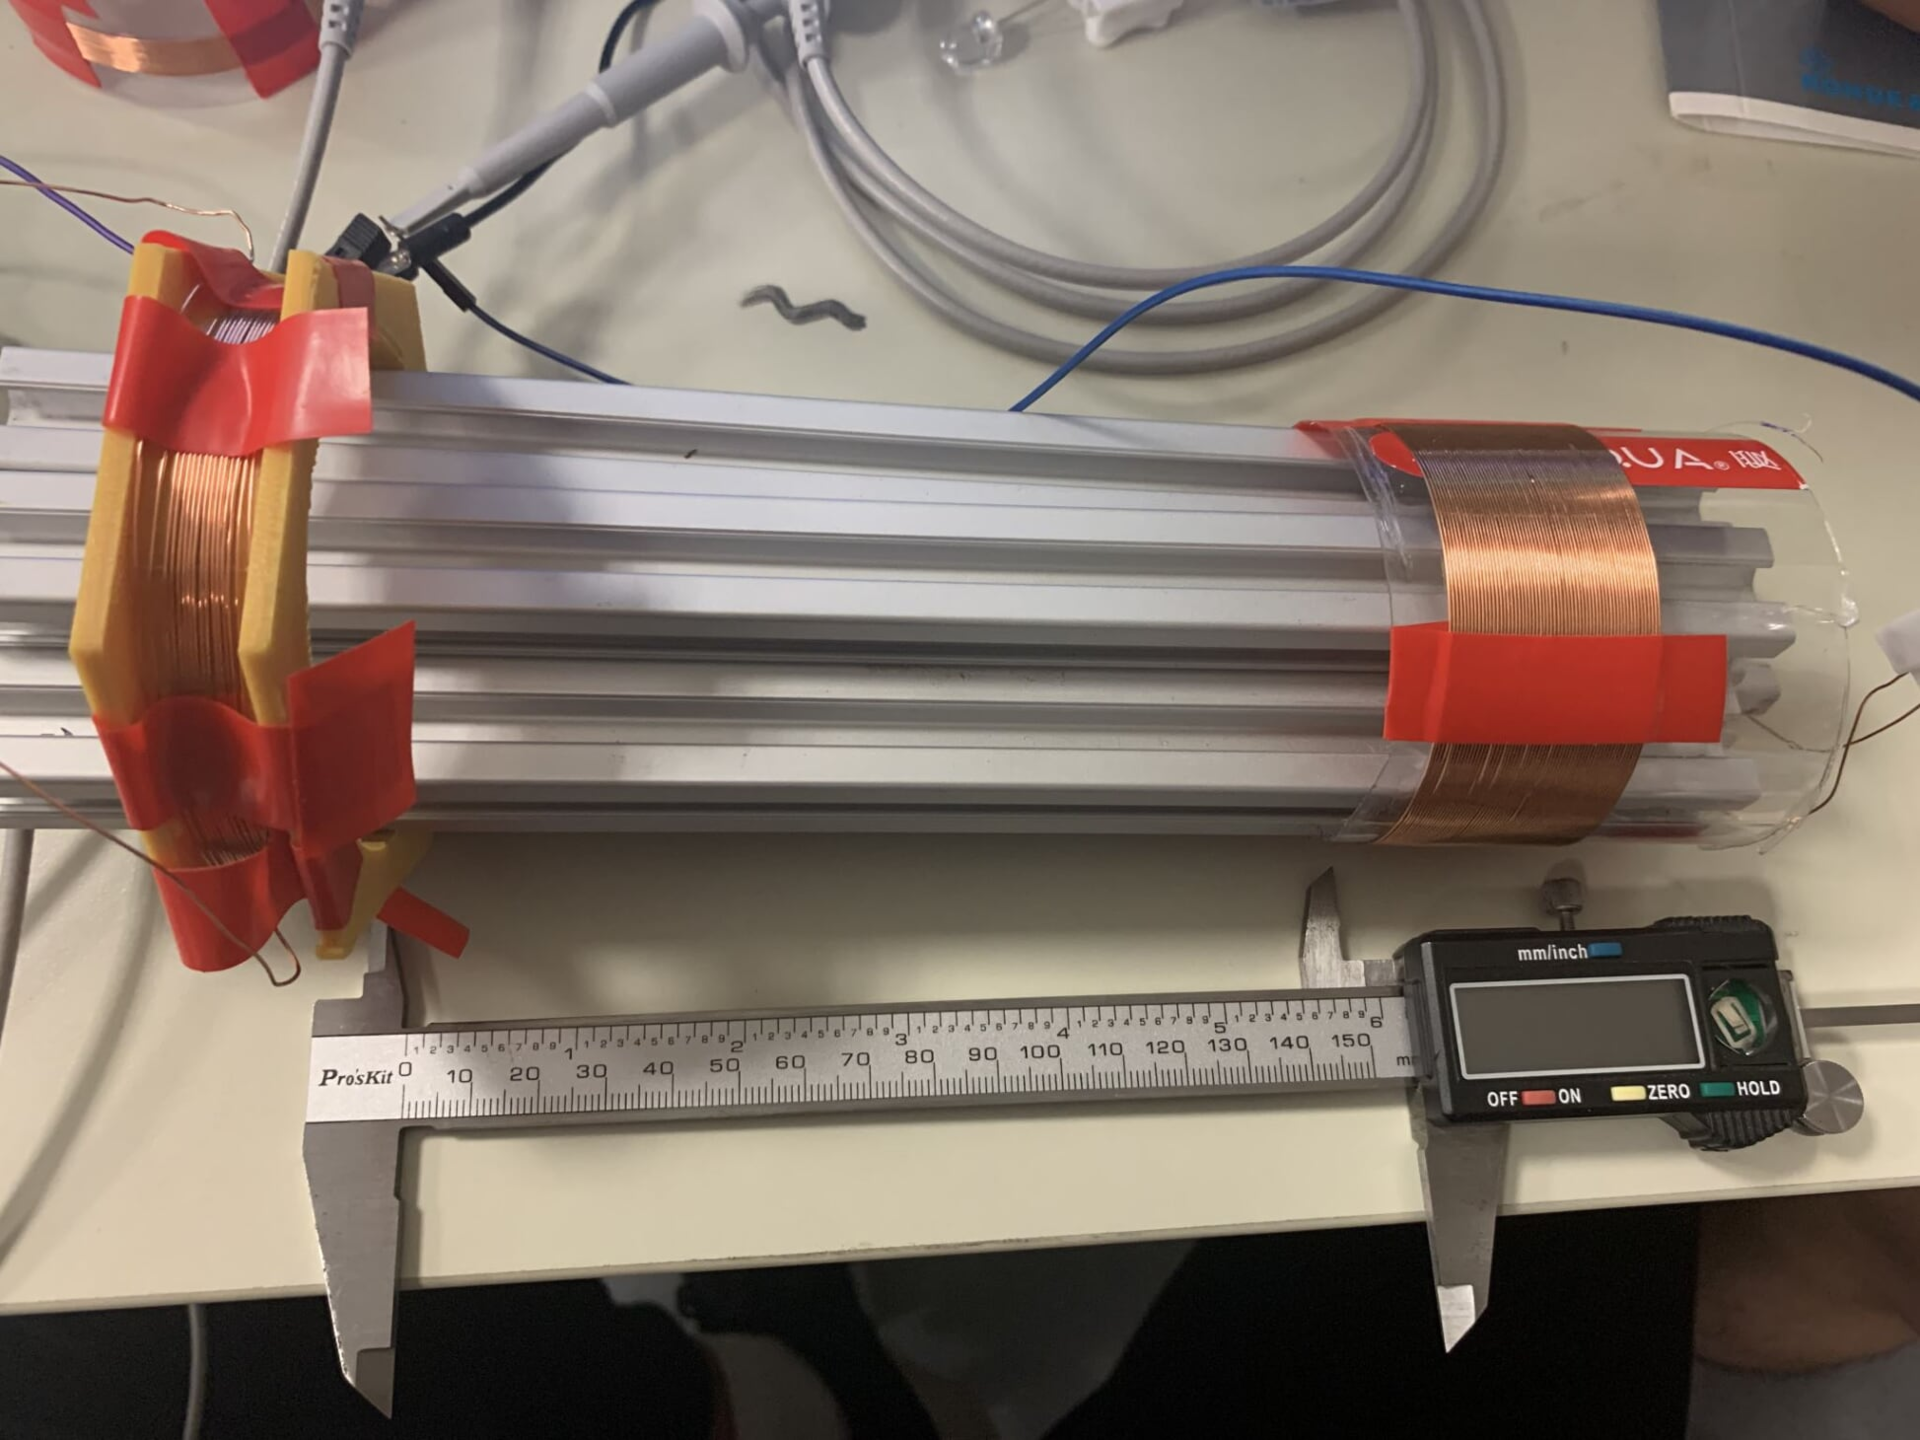
\includegraphics[scale=0.1]{频率2.png}}
        \caption{控制距离不变,插铁芯}
        \label{fig}
        \end{figure}

\begin{figure}[htbp]
        \centerline{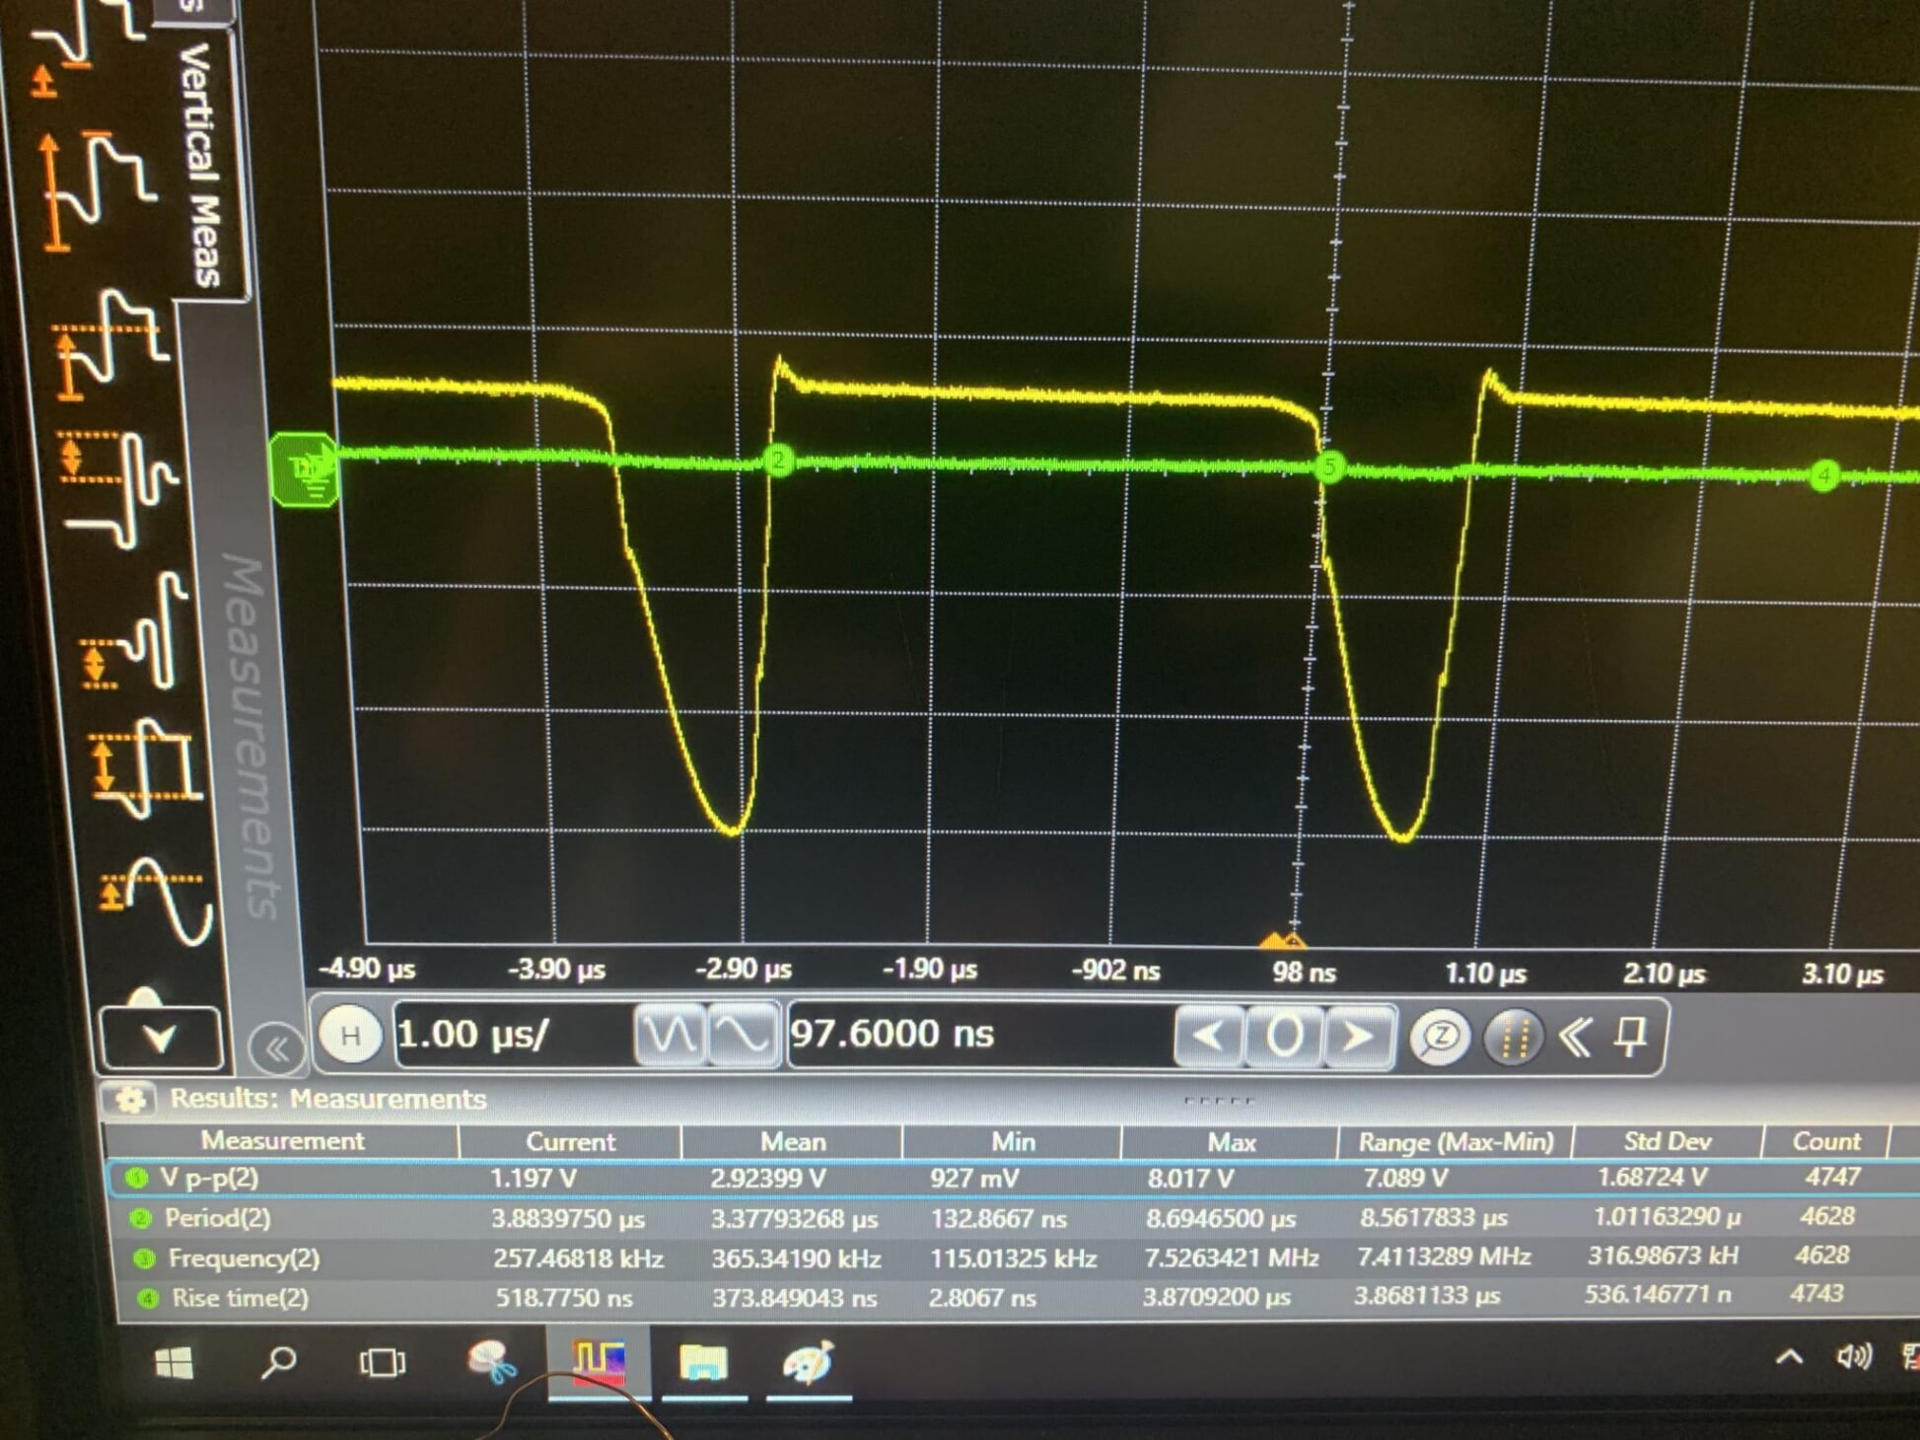
\includegraphics[scale=0.1]{频率3.png}}
        \caption{控制距离不变,插铁芯}
        \label{fig}
        \end{figure}       

\begin{figure}[htbp]
        \centerline{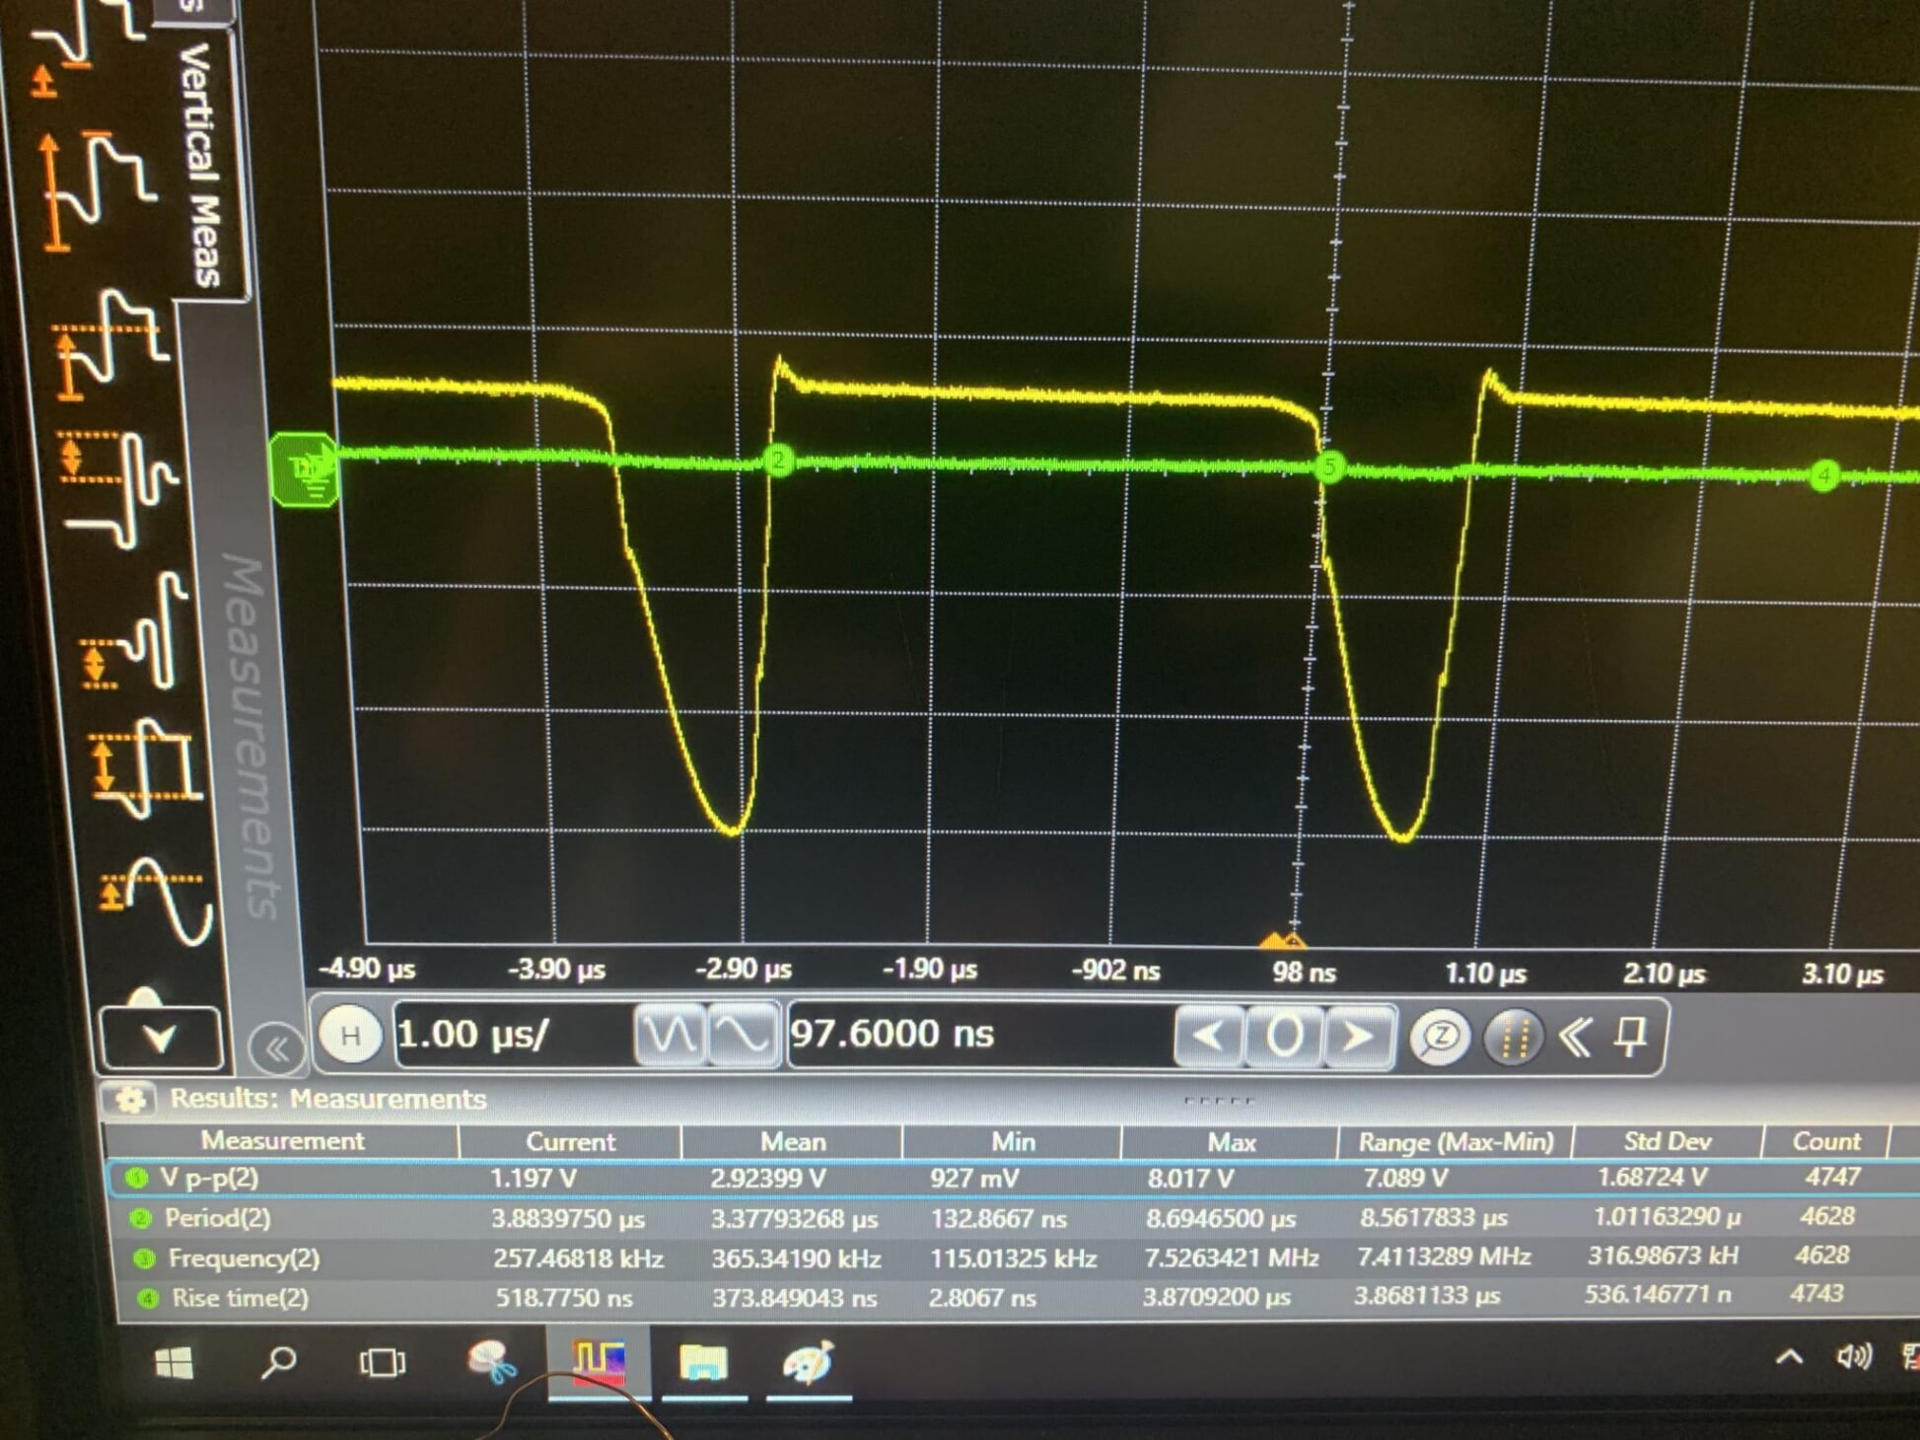
\includegraphics[scale=0.1]{频率3.png}}
        \caption{控制距离不变,插铁芯}
        \label{fig}
        \end{figure}             
        
\subsection{控制变量:线圈直径}
\subsubsection{实验设计}
本实验诣在探索接收端线圈直径对无线输电的影响,依据控制变量原则设计对照实验,只有接收端线圈直径不同。\\
\textbf{实验器材:}
\begin{itemize}
\item 发射端:直径8cm、15匝线圈
\item 接收端:1.直径5.1cm、15匝线圈  2.直径6.3cm、15匝线圈
\item 示波器
\end{itemize}
\subsubsection{实验过程}
两组都控制距离为2cm,示波器与接收线圈相连,分别观察两组实验中示波器的示数
\subsection{实验分析}
通过实验我们发现,收线圈直径为5.1cm组的电压相较于接收线圈直径为6.3cm的组低
\subsection{实验结论}
在一定范围内,增大接收端线圈直径可以提高无线输电的能力
\begin{figure}[htbp]
        \centerline{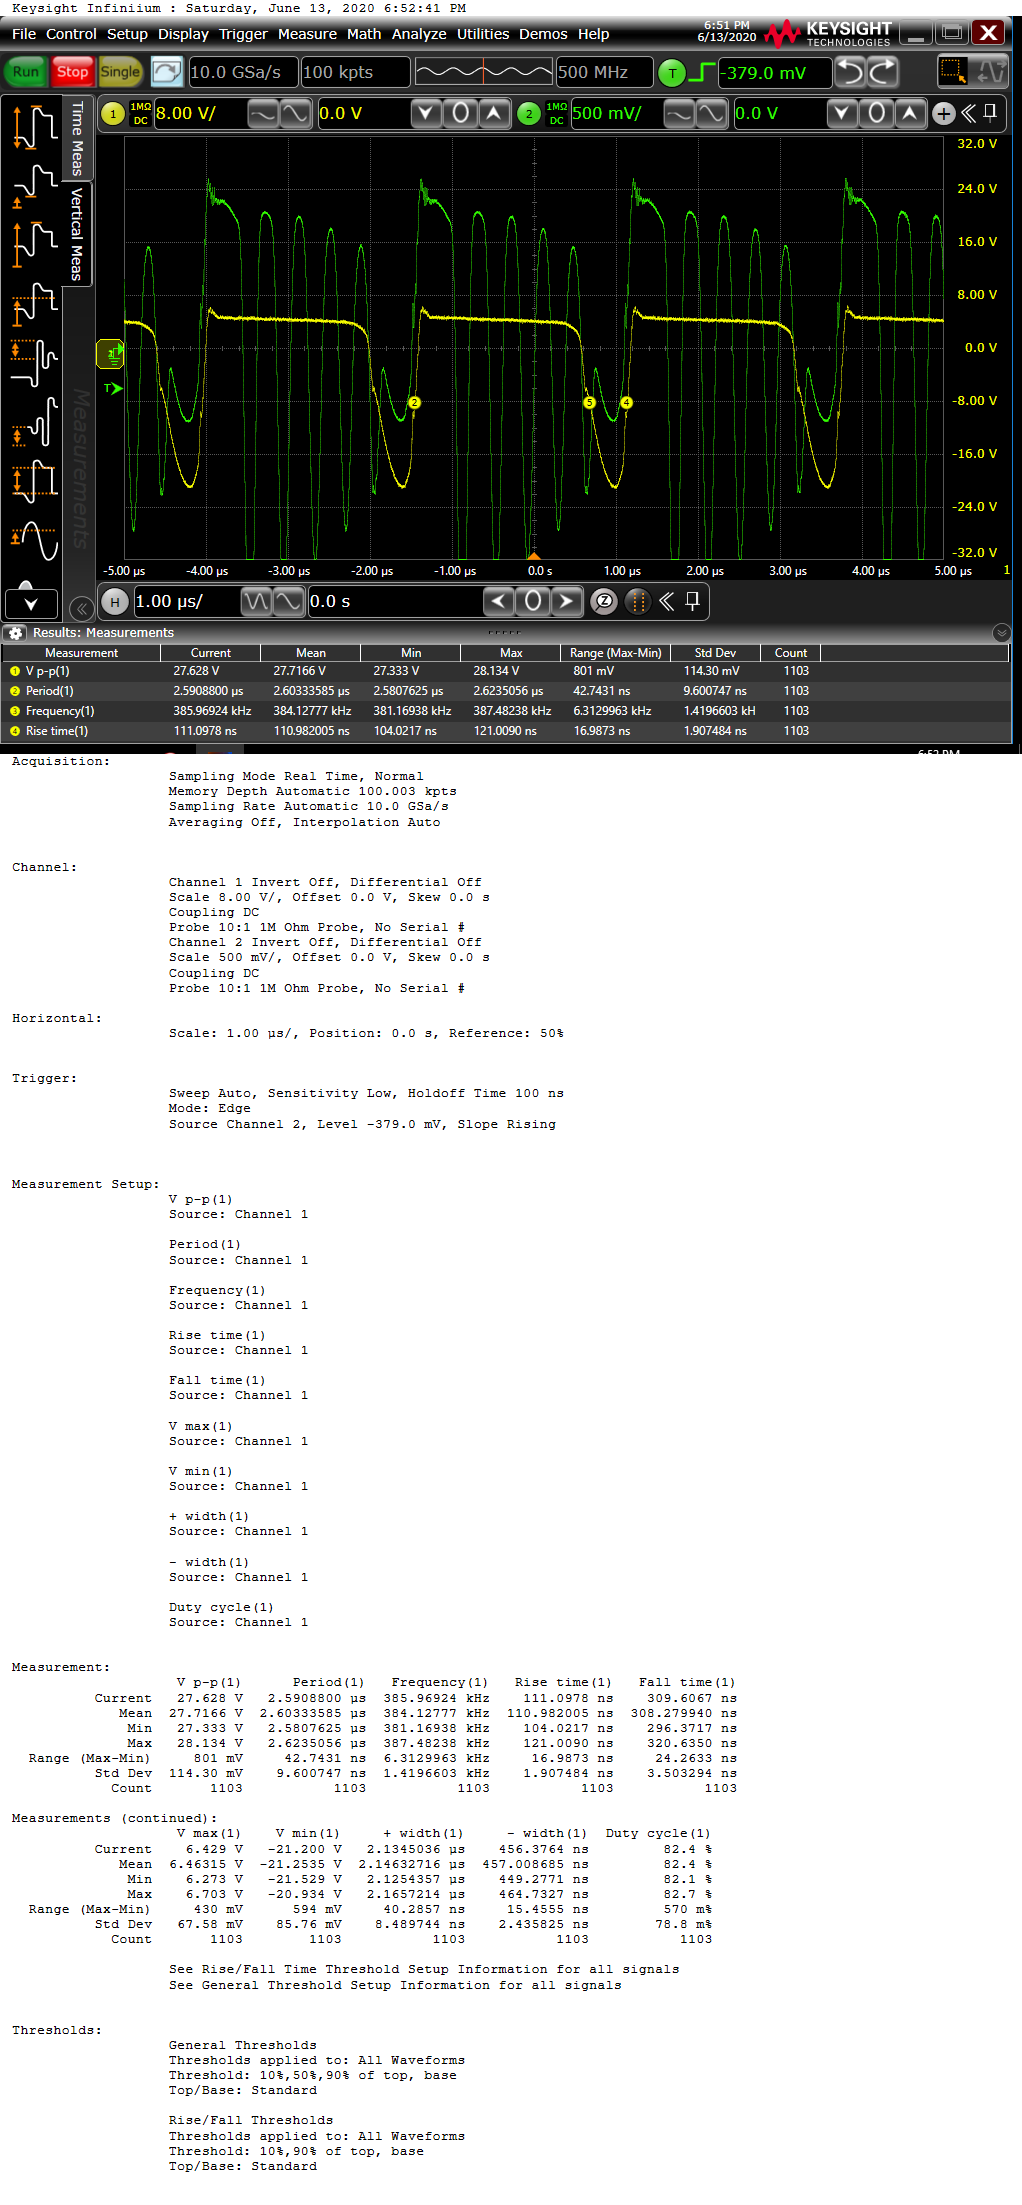
\includegraphics[scale=0.1]{z1.png}}
        \caption{直径交大组}
        \label{fig}
        \end{figure}       
\begin{figure}[htbp]
        \centerline{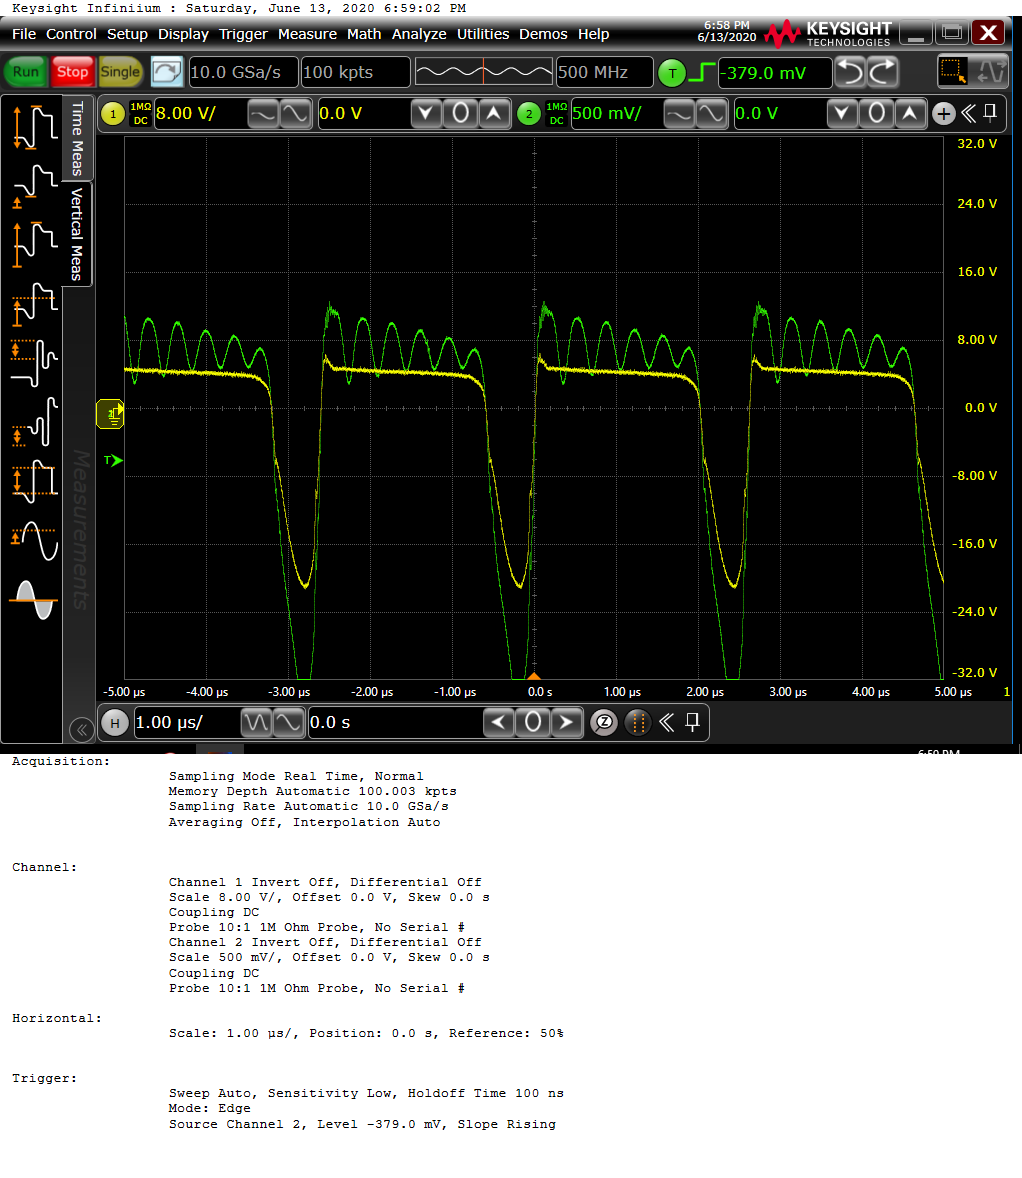
\includegraphics[scale=0.1]{z2.png}}
        \caption{直径较小组}
        \label{fig}
        \end{figure}   
\subsection{控制变量:线圈匝数}
\subsubsection{实验设计}
本实验诣在探索接收线圈的匝数对无线输电的影响,依据控制变量原则设计对照实验,只改变接收线圈匝数。
\textbf{实验器材:}
\begin{itemize}
\item 发射端:直径8cm、15匝线圈
\item 接收端:1.直径6.3cm、60匝线圈  2.直径6.3cm、30匝线圈
\item 示波器
\end{itemize}
\subsubsection{实验过程}
两组都控制距离为3cm,示波器与接收线圈相连,分别观察两组实验中示波器的示数       
\subsubsection{实验分析}
通过实验我们发现,匝数为60的组的电压比匝数为30的组的电压高
\subsubsection{实验结论}
在一定范围内,提高接收端线圈匝数可以提升无线输电的能力
\begin{figure}[htbp]
        \centerline{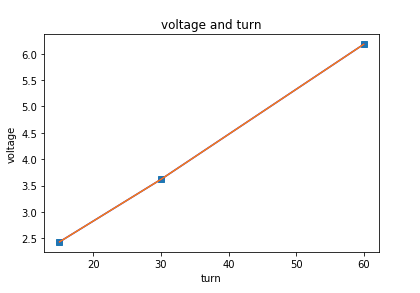
\includegraphics[scale=0.1]{匝数图.png}}
        \caption{匝数图标}
        \label{fig}
        \end{figure}
\subsection{控制变量:发射线圈与接收线圈之间角度}
\subsubsection{实验设计}
本实验诣在探索发射线圈与接收线圈之间角度对无线输电的影响,依据控制变量原则设计实验,只改变发射线圈与接收线圈之间角度。
\textbf{实验器材:}
\begin{itemize}
\item 发射端:直径8cm、15匝
\item 接收端:直径6.3cm、60匝
\item 示波器
\item 自制同心圆坐标纸
\end{itemize}
\subsubsection{实验过程}
示波器与接收线圈相连,选定直径为3cm的圆,让接收线圈沿着该圆旋转,观察示波器的示数
\subsubsection{实验分析}
通过实验我们发现当发射端线圈与接收端线圈正对时电压最大,随着二者角度增大,电压随之下降
\subsubsection{实验结论}
\begin{figure}[htbp]
        \centerline{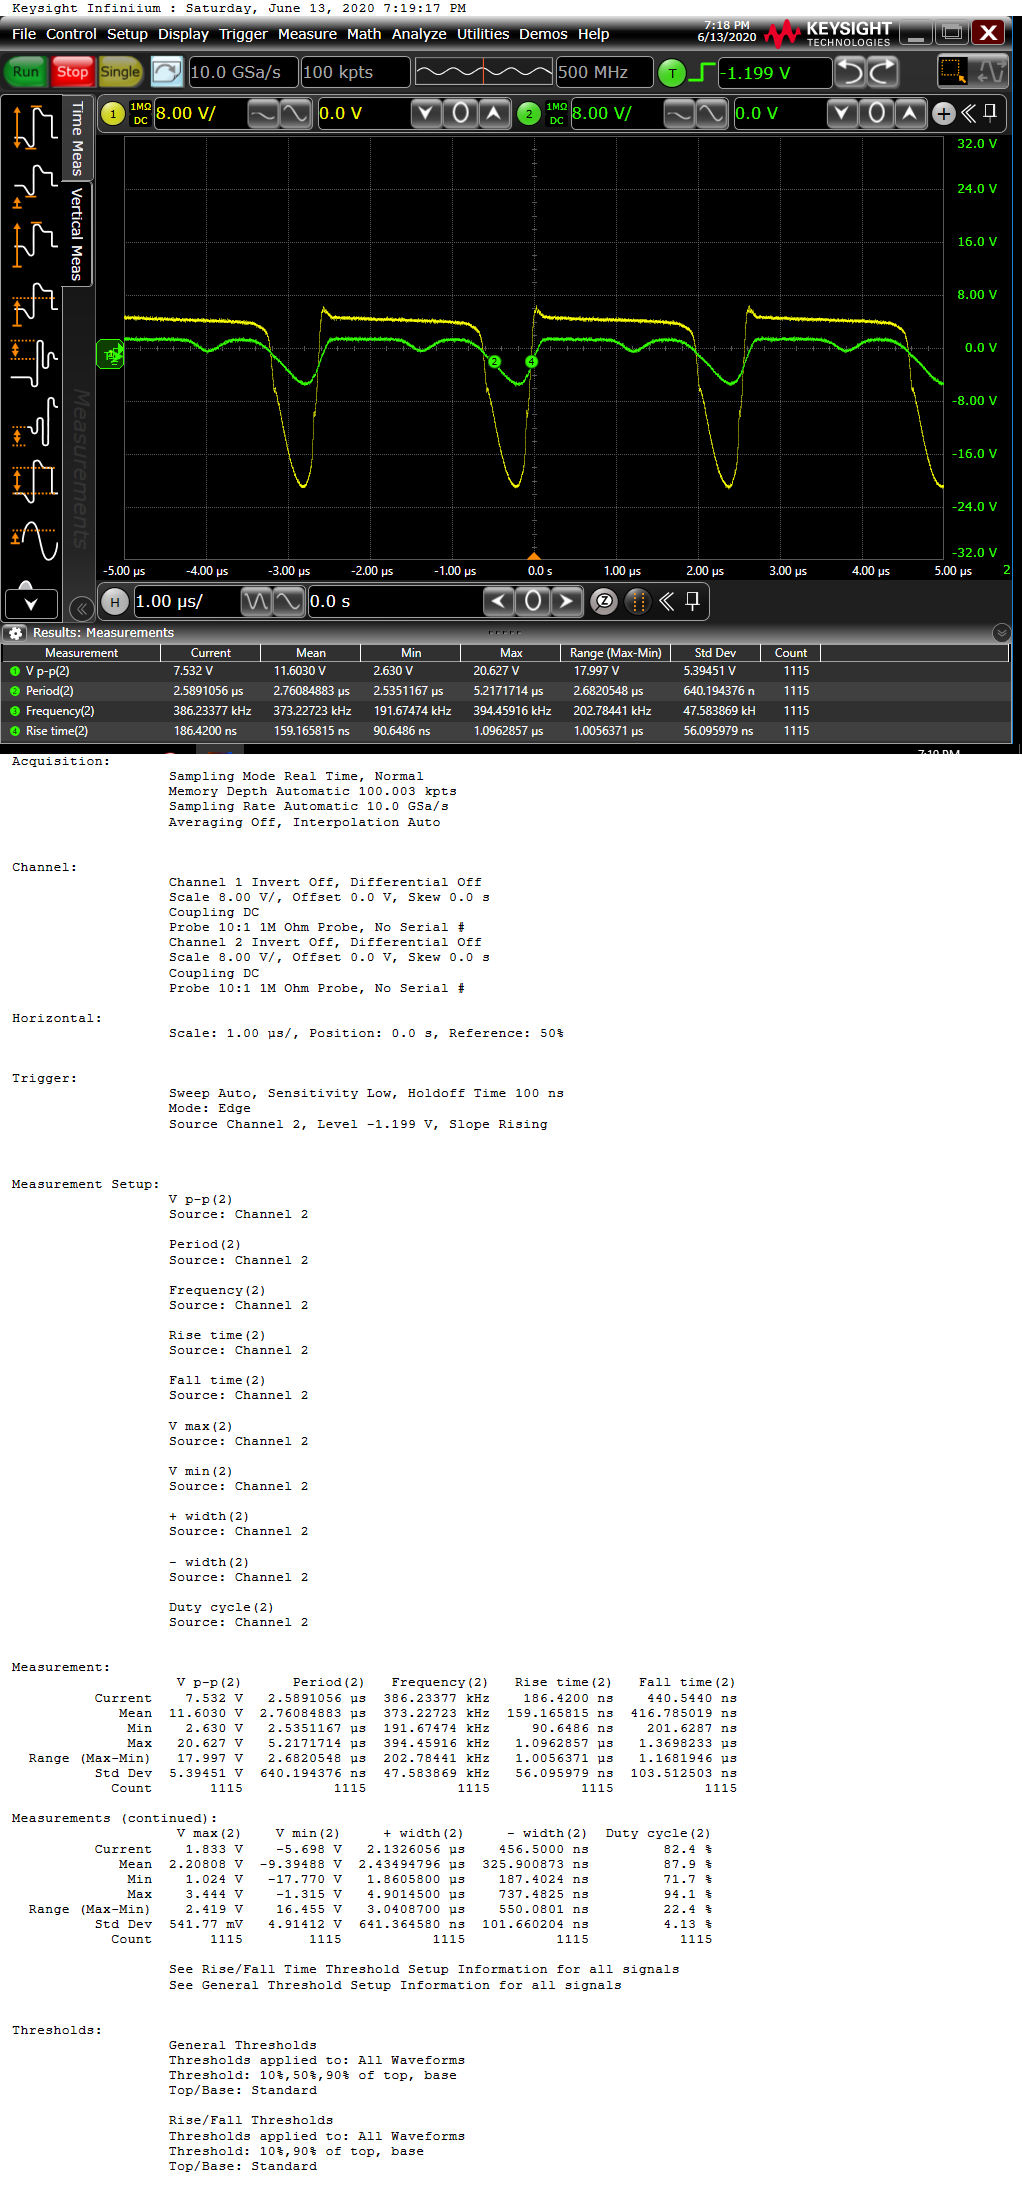
\includegraphics[scale=0.1]{角度1.png}}
        \caption{夹角较大}
        \label{fig}
        \end{figure}       
\begin{figure}[htbp]
        \centerline{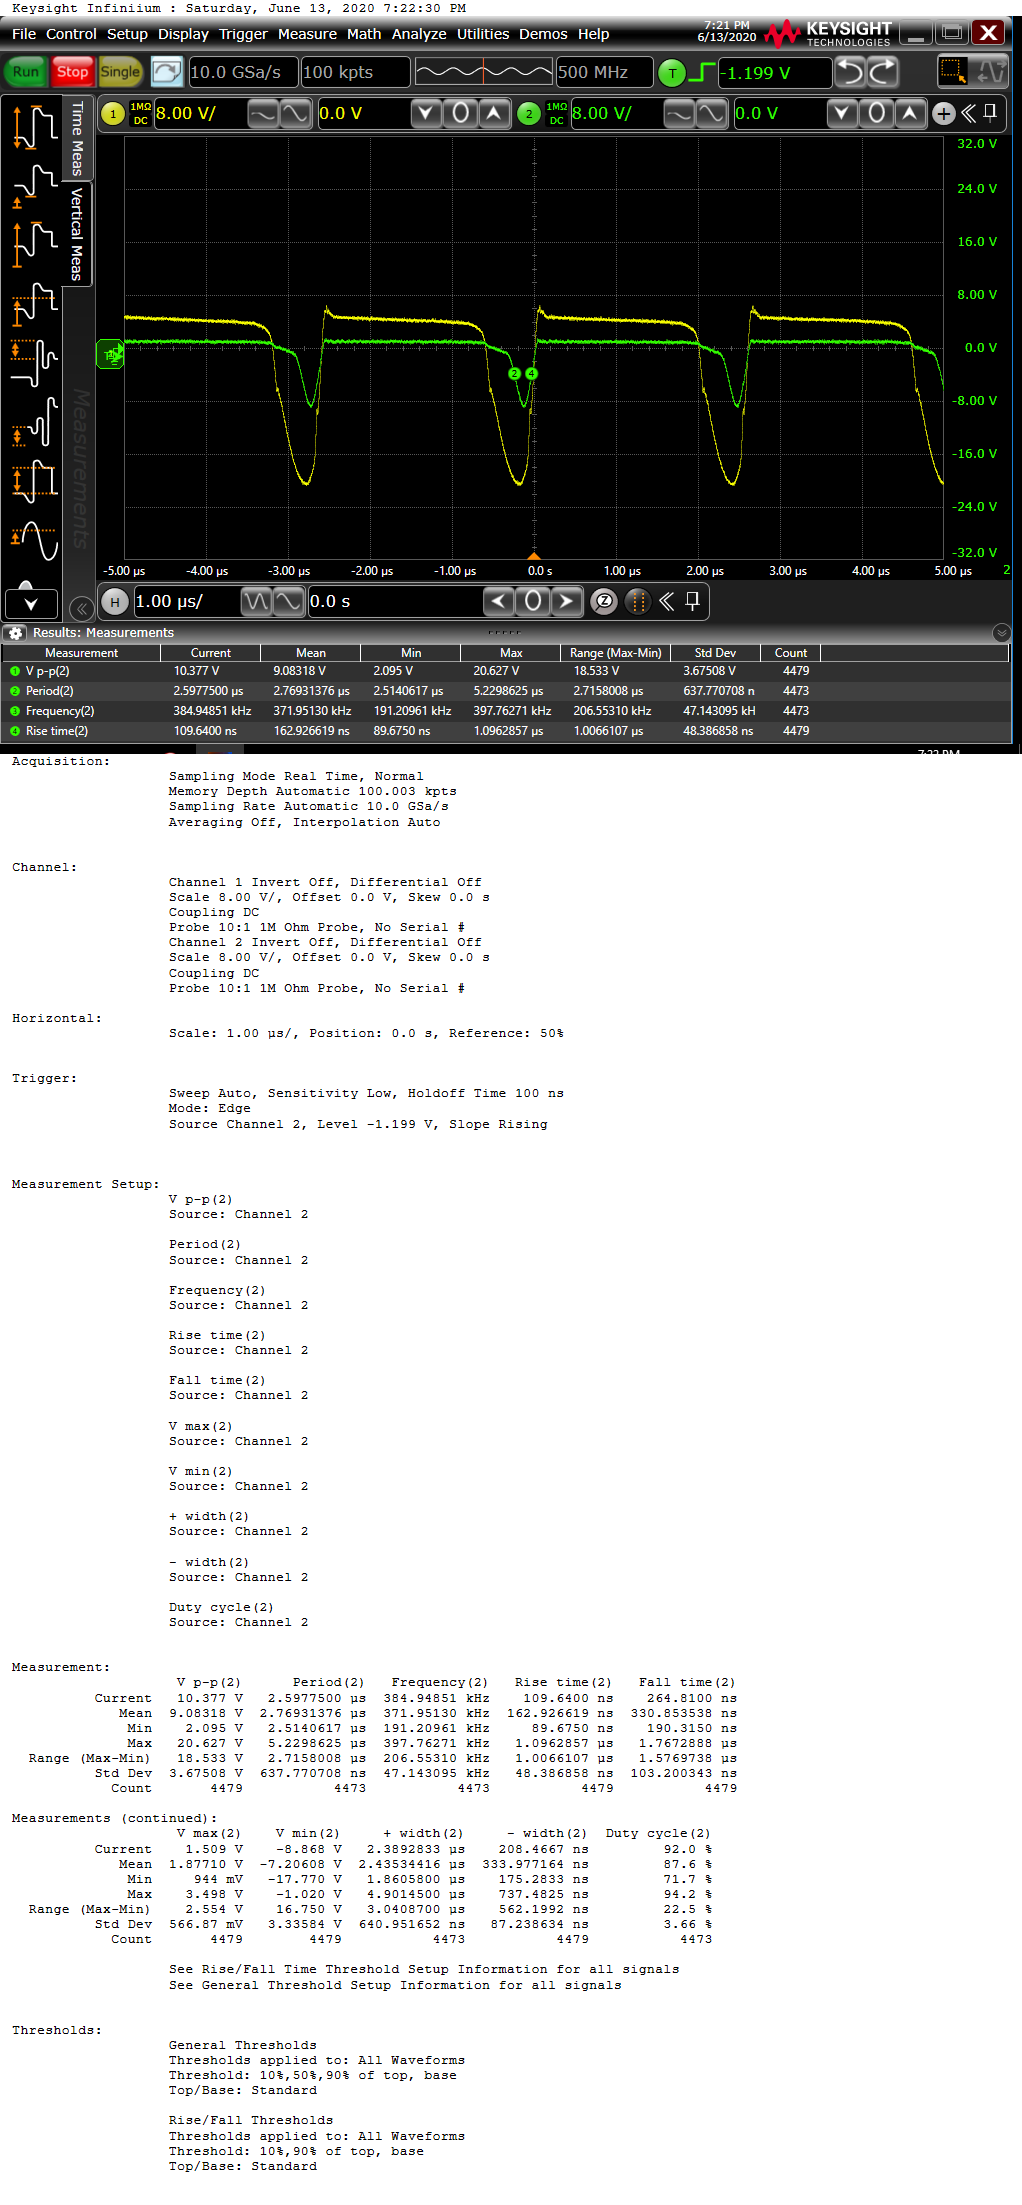
\includegraphics[scale=0.1]{角度2.png}}
        \caption{夹角较小}
        \label{fig}
        \end{figure}   
使发射端线圈与接收端线圈正对可以提升无线输电能力
\section{另一类实验设想及失败原因}
\subsection{实验设想}
通过单片机与传感器模块,进行实时的定量测量,控制五个变量,进行影响因素探究
\subsection{实验设计}
\begin{itemize}
        \item 通过超声波测距模块进行距离控制
        \item 通过角度传感器进行角度控制
        \item 通过杜邦线并联发光二极管两端与Arduino的analog端口,进行电压测量
        \item 通过霍尔传感器直接测量磁感线分布
\end{itemize}
\subsection{实验失败原因}
\begin{itemize}
        \item 由于电源模块是自激振荡模块,其频率为500khz,超出了Arduino的analog最大采样率(10000Hz),因此无法进行电压测量
        \item 霍尔传感器的测量面积太小,无明显现象
\end{itemize}
\subsection{其它}
\begin{itemize}
        \item   由于霍尔传感器与单片机模拟输入方案的失败,超声波测距传感器并未比游标卡尺方案更便利,因此我们组决定抛弃此方案
        \item   购入的角度传感器型号为 SW520D,其实质为倾斜传感器,未达到我们组的要求,因此该方案被弃用。
\end{itemize}

\section{拓展实验:霍尔电机测速}
\subsection{实验原理}
\begin{itemize}
        \item 霍尔传感器可以测量其感应元件测量极附近的磁通量。我们组选用的基于A3144非线性霍尔传感器与S49E线性传感器的霍尔模块均可以让霍尔信号经过比较器输出一个数字量(即高电平)
        \item 当带有磁性的物品(例如电机带动的叶片末端,和我们进行模拟的surface pen)接近霍尔传感器时,其IO口会输出一个高电平信号,此时记录时间t1。
        \item 当电机完成一次转动后,霍尔传感器IO口会再次输出一个高电平信号,记录时间t2
\end{itemize}
则其转速为 $ \frac{1}{t_1 - t_2} \\ \frac{rad}{s}$ \\
\textbf{相应代码见附录}
\begin{figure}[htbp]
        \centerline{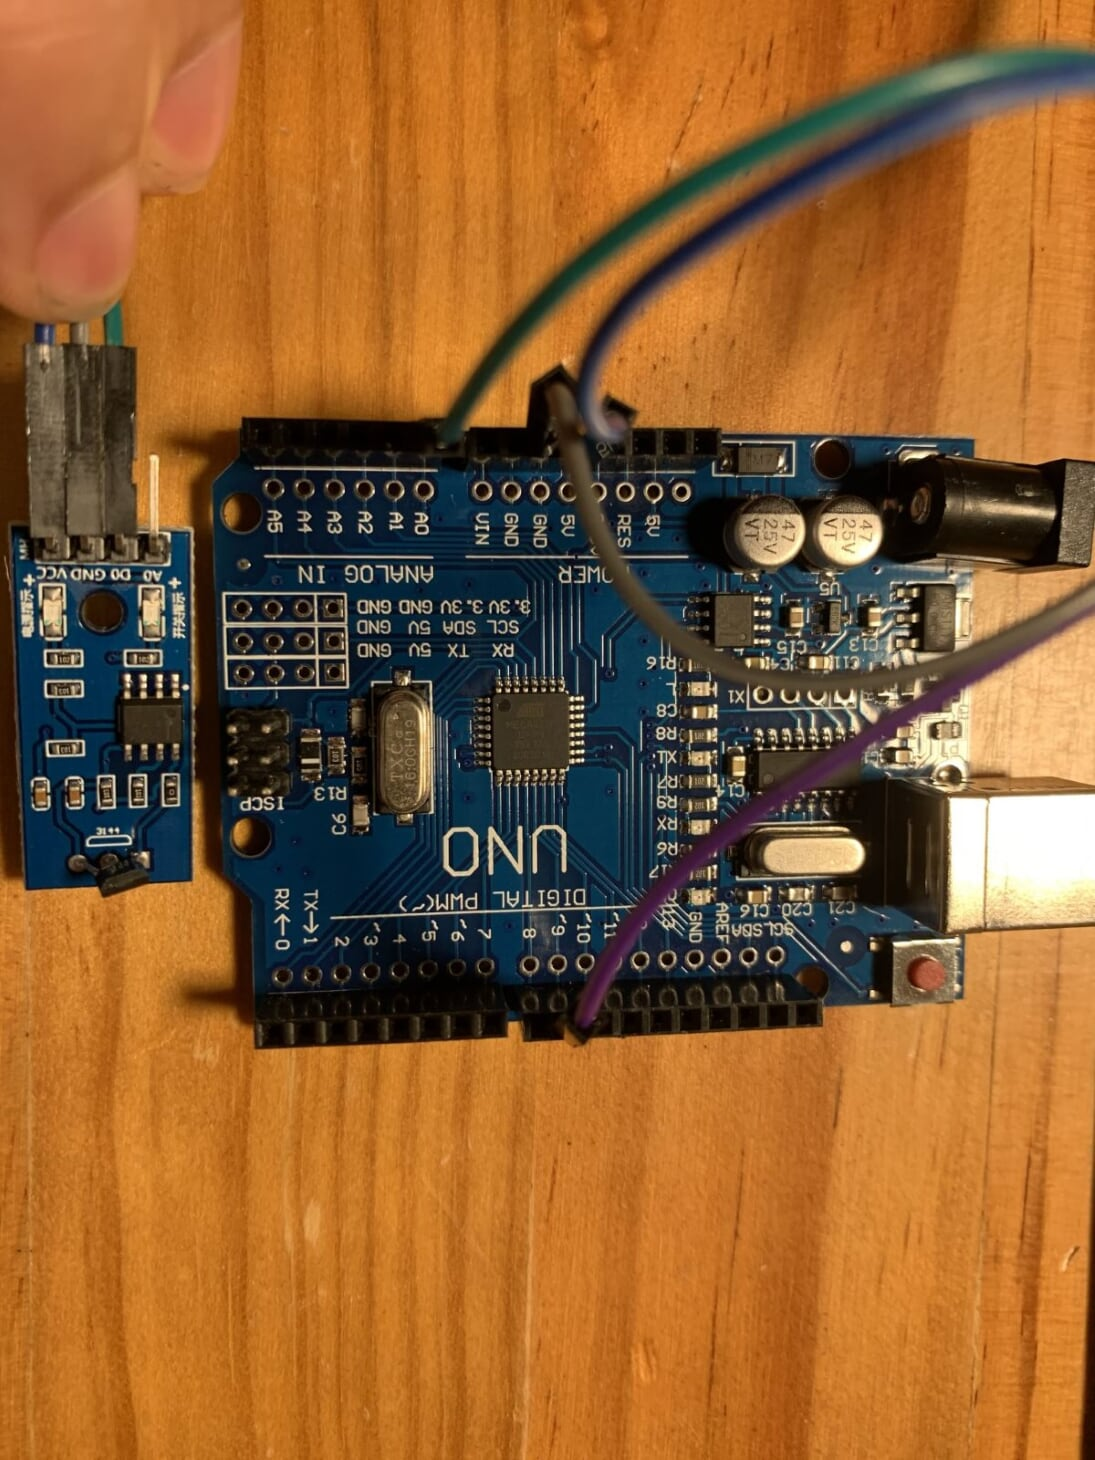
\includegraphics[scale=0.1]{霍尔.png}}
        \caption{霍尔测速器电路搭建}
        \label{fig}
        \end{figure}
\vspace{12pt}
\newpage
\section{附录}
\subsection{超声波距离传感器代码}
\begin{lstlisting}
        const int TRIG = 5;
        const int ECHO = 6;
        const int A_0   = A1;
        const int D_0   = A0;
        
        void setup() {
          // put your setup code here, to run once:
          pinMode(TRIG, OUTPUT);
          pinMode(ECHO, INPUT);
          Serial.begin(9600);
        }
        
        void Distance() {
          int duration, distance;
          digitalWrite(TRIG, LOW);
          delayMicroseconds(2);
          // Sets the TRIG on HIGH state for 10 micro seconds
          digitalWrite(TRIG, HIGH);
          delayMicroseconds(10);
          digitalWrite(TRIG, LOW);
          // Reads the ECHO, returns the sound wave travel time in microseconds
          duration = pulseIn(ECHO, HIGH);
          // Calculating the distance
          distance = duration * 0.034 / 2;
          // Prints the distance on the Serial Monitor
          Serial.print("Distance: ");
          Serial.print(distance);
          Serial.println("cm");
        }
        
        
        
        void loop() {
          Serial.println("Begin");
         Distance();
        }
                                             
\end{lstlisting}

\subsection{霍尔测速器}
\begin{lstlisting}
        const int G_0 = 9;
        int period = 0;
        int flag = 0;
        float R = 0.3; // 30cm
        const int debug = 0;
        int Delay = 100;
        
        void setup()
        {
          Serial.begin(9600);
          pinMode(G_0, INPUT);
        
        }
        
        void loop() {
          if ( digitalRead(G_0) == HIGH ) {
            if (flag == 0){
            if(debug){
                Serial.println("-------------");
                Serial.println("Begin Measure");;
                Serial.println("-------------");
             }
        
        
              
              delay(Delay);
              period += Delay;
              flag =1;
            }
            else{
              double tmp1 = 2.0  * R  * 1000.0 / period * PI;
              float tmp2 = 1000.0 / period;
              //float tmp2 = period / 1000;
              
              if(debug){
                Serial.println("-------------");
                Serial.print("time: ");
                Serial.println(period);
                Serial.println("-------------");
              }
              if(!debug) Serial.println("-------------------");
              Serial.println("The current speed is: ");
              Serial.print(tmp1);
              Serial.println(" m/s ");
              Serial.println("The current turning speed is: ");
              Serial.print(tmp2);
              Serial.println(" round/s ");
              if(!debug) Serial.println("-------------------");
              period = 0;
              delay(Delay);
              period += Delay;
            }
          }
          if(flag){
            delay(5);
            period += 5;
          }
        }
\end{lstlisting}
\subsection{磁通量}
\begin{lstlisting}
        const int A_0 = A0;

void setup()
{
  Serial.begin(9600);


}

void loop(){
  Serial.println(analogRead(A_0));
  delay(300);
}
\end{lstlisting}
\subsection{电感}
\begin{lstlisting}
        import numpy as np
        from scipy import interpolate
        import matplotlib.pyplot as pyplot
        import math
        
        print('''
        -------------------------------------------------------
        
                     电感计算器
        
        -------------------------------------------------------
        ''')
        
        print("请输入半径 (m) :")
        R = input()
        try:
                R = float(R)
        except:
                print("输入不合法.")
        
        
        print("请输入螺线管长度 (m) :")
        L = input()
        try:
                L = float(L)
        except:
                print("输入不合法.")
        
        
        # print("请输入线圈匝数:")
        N = L // 0.00049
        # try:
        #         N = float(N)
        # except:
        #         print("输入不合法.")
        
        
        x = np.array([0.1, 0.2, 0.3, 0.4, 0.6, 0.8, 1.0, 1.5, 2.0, 3.0, 4.0, 5.0, 10, 20])
        y = np.array([0.96, 0.92, 0.88, 0.85, 0.79, 0.74, 0.69, 0.60, 0.52, 0.43, 0.37, 0.32, 0.2, 0.12])
        f = interpolate.interp1d(x, y, kind = 'cubic')
        
        S = R ** 2 * math.pi
        mu = 4 * math.pi * 1e-7
        k = f(2 * R / L)
        H = k * mu * (N ** 2) * S / L
        
        print('''
        --------------------------------------------------
        The answer is 
        ''', end='')
        print(H, end=' H')
        print('''
        --------------------------------------------------
        ''')                                            
        
        
        
\end{lstlisting} 
\end{document}

